%% bare_jrnl_compsoc.tex
%% V1.3
%% 2007/01/11
%% by Michael Shell
%% See:
%% http://www.michaelshell.org/
%% for current contact information.
%%
%% This is a skeleton file demonstrating the use of IEEEtran.cls
%% (requires IEEEtran.cls version 1.7 or later) with an IEEE Computer
%% Society journal paper.
%%
%% Support sites:
%% http://www.michaelshell.org/tex/ieeetran/
%% http://www.ctan.org/tex-archive/macros/latex/contrib/IEEEtran/
%% and
%% http://www.ieee.org/

%%*************************************************************************
%% Legal Notice:
%% This code is offered as-is without any warranty either expressed or
%% implied; without even the implied warranty of MERCHANTABILITY or
%% FITNESS FOR A PARTICULAR PURPOSE!
%% User assumes all risk.
%% In no event shall IEEE or any contributor to this code be liable for
%% any damages or losses, including, but not limited to, incidental,
%% consequential, or any other damages, resulting from the use or misuse
%% of any information contained here.
%%
%% All comments are the opinions of their respective authors and are not
%% necessarily endorsed by the IEEE.
%%
%% This work is distributed under the LaTeX Project Public License (LPPL)
%% ( http://www.latex-project.org/ ) version 1.3, and may be freely used,
%% distributed and modified. A copy of the LPPL, version 1.3, is included
%% in the base LaTeX documentation of all distributions of LaTeX released
%% 2003/12/01 or later.
%% Retain all contribution notices and credits.
%% ** Modified files should be clearly indicated as such, including  **
%% ** renaming them and changing author support contact information. **
%%
%% File list of work: IEEEtran.cls, IEEEtran_HOWTO.pdf, bare_adv.tex,
%%                    bare_conf.tex, bare_jrnl.tex, bare_jrnl_compsoc.tex
%%*************************************************************************

% *** Authors should verify (and, if needed, correct) their LaTeX system  ***
% *** with the testflow diagnostic prior to trusting their LaTeX platform ***
% *** with production work. IEEE's font choices can trigger bugs that do  ***
% *** not appear when using other class files.                            ***
% The testflow support page is at:
% http://www.michaelshell.org/tex/testflow/




% Note that the a4paper option is mainly intended so that authors in
% countries using A4 can easily print to A4 and see how their papers will
% look in print - the typesetting of the document will not typically be
% affected with changes in paper size (but the bottom and side margins will).
% Use the testflow package mentioned above to verify correct handling of
% both paper sizes by the user's LaTeX system.
%
% Also note that the "draftcls" or "draftclsnofoot", not "draft", option
% should be used if it is desired that the figures are to be displayed in
% draft mode.
%
% The Computer Society usually requires 10pt for submissions.
%
\documentclass[10pt,journal,cspaper,compsoc]{IEEEtran}
% \documentclass[10pt,journal,draftclsnofoot,onecolumn]{IEEEtran}
%
% If IEEEtran.cls has not been installed into the LaTeX system files,
% manually specify the path to it like:
% \documentclass[12pt,journal,compsoc]{../sty/IEEEtran}





% Some very useful LaTeX packages include:
% (uncomment the ones you want to load)


% *** MISC UTILITY PACKAGES ***
%
%\usepackage{ifpdf}
% Heiko Oberdiek's ifpdf.sty is very useful if you need conditional
% compilation based on whether the output is pdf or dvi.
% usage:
% \ifpdf
%   % pdf code
% \else
%   % dvi code
% \fi
% The latest version of ifpdf.sty can be obtained from:
% http://www.ctan.org/tex-archive/macros/latex/contrib/oberdiek/
% Also, note that IEEEtran.cls V1.7 and later provides a builtin
% \ifCLASSINFOpdf conditional that works the same way.
% When switching from latex to pdflatex and vice-versa, the compiler may
% have to be run twice to clear warning/error messages.






% *** CITATION PACKAGES ***
%
\ifCLASSOPTIONcompsoc
  % IEEE Computer Society needs nocompress option
  % requires cite.sty v4.0 or later (November 2003)
  % \usepackage[nocompress]{cite}
\else
  % normal IEEE
  % \usepackage{cite}
\fi
% cite.sty was written by Donald Arseneau
% V1.6 and later of IEEEtran pre-defines the format of the cite.sty package
% \cite{} output to follow that of IEEE. Loading the cite package will
% result in citation numbers being automatically sorted and properly
% "compressed/ranged". e.g., [1], [9], [2], [7], [5], [6] without using
% cite.sty will become [1], [2], [5]--[7], [9] using cite.sty. cite.sty's
% \cite will automatically add leading space, if needed. Use cite.sty's
% noadjust option (cite.sty V3.8 and later) if you want to turn this off.
% cite.sty is already installed on most LaTeX systems. Be sure and use
% version 4.0 (2003-05-27) and later if using hyperref.sty. cite.sty does
% not currently provide for hyperlinked citations.
% The latest version can be obtained at:
% http://www.ctan.org/tex-archive/macros/latex/contrib/cite/
% The documentation is contained in the cite.sty file itself.
%
% Note that some packages require special options to format as the Computer
% Society requires. In particular, Computer Society  papers do not use
% compressed citation ranges as is done in typical IEEE papers
% (e.g., [1]-[4]). Instead, they list every citation separately in order
% (e.g., [1], [2], [3], [4]). To get the latter we need to load the cite
% package with the nocompress option which is supported by cite.sty v4.0
% and later. Note also the use of a CLASSOPTION conditional provided by
% IEEEtran.cls V1.7 and later.





% *** GRAPHICS RELATED PACKAGES ***
%
\ifCLASSINFOpdf
  \usepackage[pdftex]{graphicx}
  \usepackage{subfigure}
  \usepackage{algorithm}
  \usepackage{algorithmic}
  \usepackage{multirow}
  \usepackage{threeparttable}
  \newcommand{\specialcell}[2][c]{\begin{tabular}[#1]{@{}c@{}}#2\end{tabular}}
  % declare the path(s) where your graphic files are
  % \graphicspath{{../pdf/}{../jpeg/}}
  % and their extensions so you won't have to specify these with
  % every instance of \includegraphics
  % \DeclareGraphicsExtensions{.pdf,.jpeg,.png}
\else
  % or other class option (dvipsone, dvipdf, if not using dvips). graphicx
  % will default to the driver specified in the system graphics.cfg if no
  % driver is specified.
  % \usepackage[dvips]{graphicx}
  % declare the path(s) where your graphic files are
  % \graphicspath{{../eps/}}
  % and their extensions so you won't have to specify these with
  % every instance of \includegraphics
  % \DeclareGraphicsExtensions{.eps}
\fi
% graphicx was written by David Carlisle and Sebastian Rahtz. It is
% required if you want graphics, photos, etc. graphicx.sty is already
% installed on most LaTeX systems. The latest version and documentation can
% be obtained at:
% http://www.ctan.org/tex-archive/macros/latex/required/graphics/
% Another good source of documentation is "Using Imported Graphics in
% LaTeX2e" by Keith Reckdahl which can be found as epslatex.ps or
% epslatex.pdf at: http://www.ctan.org/tex-archive/info/
%
% latex, and pdflatex in dvi mode, support graphics in encapsulated
% postscript (.eps) format. pdflatex in pdf mode supports graphics
% in .pdf, .jpeg, .png and .mps (metapost) formats. Users should ensure
% that all non-photo figures use a vector format (.eps, .pdf, .mps) and
% not a bitmapped formats (.jpeg, .png). IEEE frowns on bitmapped formats
% which can result in "jaggedy"/blurry rendering of lines and letters as
% well as large increases in file sizes.
%
% You can find documentation about the pdfTeX application at:
% http://www.tug.org/applications/pdftex





% *** MATH PACKAGES ***
%
%\usepackage[cmex10]{amsmath}
% A popular package from the American Mathematical Society that provides
% many useful and powerful commands for dealing with mathematics. If using
% it, be sure to load this package with the cmex10 option to ensure that
% only type 1 fonts will utilized at all point sizes. Without this option,
% it is possible that some math symbols, particularly those within
% footnotes, will be rendered in bitmap form which will result in a
% document that can not be IEEE Xplore compliant!
%
% Also, note that the amsmath package sets \interdisplaylinepenalty to 10000
% thus preventing page breaks from occurring within multiline equations. Use:
%\interdisplaylinepenalty=2500
% after loading amsmath to restore such page breaks as IEEEtran.cls normally
% does. amsmath.sty is already installed on most LaTeX systems. The latest
% version and documentation can be obtained at:
% http://www.ctan.org/tex-archive/macros/latex/required/amslatex/math/





% *** SPECIALIZED LIST PACKAGES ***
%
%\usepackage{algorithmic}
% algorithmic.sty was written by Peter Williams and Rogerio Brito.
% This package provides an algorithmic environment fo describing algorithms.
% You can use the algorithmic environment in-text or within a figure
% environment to provide for a floating algorithm. Do NOT use the algorithm
% floating environment provided by algorithm.sty (by the same authors) or
% algorithm2e.sty (by Christophe Fiorio) as IEEE does not use dedicated
% algorithm float types and packages that provide these will not provide
% correct IEEE style captions. The latest version and documentation of
% algorithmic.sty can be obtained at:
% http://www.ctan.org/tex-archive/macros/latex/contrib/algorithms/
% There is also a support site at:
% http://algorithms.berlios.de/index.html
% Also of interest may be the (relatively newer and more customizable)
% algorithmicx.sty package by Szasz Janos:
% http://www.ctan.org/tex-archive/macros/latex/contrib/algorithmicx/




% *** ALIGNMENT PACKAGES ***
%
%\usepackage{array}
% Frank Mittelbach's and David Carlisle's array.sty patches and improves
% the standard LaTeX2e array and tabular environments to provide better
% appearance and additional user controls. As the default LaTeX2e table
% generation code is lacking to the point of almost being broken with
% respect to the quality of the end results, all users are strongly
% advised to use an enhanced (at the very least that provided by array.sty)
% set of table tools. array.sty is already installed on most systems. The
% latest version and documentation can be obtained at:
% http://www.ctan.org/tex-archive/macros/latex/required/tools/


%\usepackage{mdwmath}
%\usepackage{mdwtab}
% Also highly recommended is Mark Wooding's extremely powerful MDW tools,
% especially mdwmath.sty and mdwtab.sty which are used to format equations
% and tables, respectively. The MDWtools set is already installed on most
% LaTeX systems. The lastest version and documentation is available at:
% http://www.ctan.org/tex-archive/macros/latex/contrib/mdwtools/


% IEEEtran contains the IEEEeqnarray family of commands that can be used to
% generate multiline equations as well as matrices, tables, etc., of high
% quality.


%\usepackage{eqparbox}
% Also of notable interest is Scott Pakin's eqparbox package for creating
% (automatically sized) equal width boxes - aka "natural width parboxes".
% Available at:
% http://www.ctan.org/tex-archive/macros/latex/contrib/eqparbox/





% *** SUBFIGURE PACKAGES ***
%\ifCLASSOPTIONcompsoc
%\usepackage[tight,normalsize,sf,SF]{subfigure}
%\else
%\usepackage[tight,footnotesize]{subfigure}
%\fi
% subfigure.sty was written by Steven Douglas Cochran. This package makes it
% easy to put subfigures in your figures. e.g., "Figure 1a and 1b". For IEEE
% work, it is a good idea to load it with the tight package option to reduce
% the amount of white space around the subfigures. Computer Society papers
% use a larger font and \sffamily font for their captions, hence the
% additional options needed under compsoc mode. subfigure.sty is already
% installed on most LaTeX systems. The latest version and documentation can
% be obtained at:
% http://www.ctan.org/tex-archive/obsolete/macros/latex/contrib/subfigure/
% subfigure.sty has been superceeded by subfig.sty.


%\ifCLASSOPTIONcompsoc
%  \usepackage[caption=false]{caption}
%  \usepackage[font=normalsize,labelfont=sf,textfont=sf]{subfig}
%\else
%  \usepackage[caption=false]{caption}
%  \usepackage[font=footnotesize]{subfig}
%\fi
% subfig.sty, also written by Steven Douglas Cochran, is the modern
% replacement for subfigure.sty. However, subfig.sty requires and
% automatically loads Axel Sommerfeldt's caption.sty which will override
% IEEEtran.cls handling of captions and this will result in nonIEEE style
% figure/table captions. To prevent this problem, be sure and preload
% caption.sty with its "caption=false" package option. This is will preserve
% IEEEtran.cls handing of captions. Version 1.3 (2005/06/28) and later
% (recommended due to many improvements over 1.2) of subfig.sty supports
% the caption=false option directly:
%\ifCLASSOPTIONcompsoc
%  \usepackage[caption=false,font=normalsize,labelfont=sf,textfont=sf]{subfig}
%\else
%  \usepackage[caption=false,font=footnotesize]{subfig}
%\fi
%
% The latest version and documentation can be obtained at:
% http://www.ctan.org/tex-archive/macros/latex/contrib/subfig/
% The latest version and documentation of caption.sty can be obtained at:
% http://www.ctan.org/tex-archive/macros/latex/contrib/caption/




% *** FLOAT PACKAGES ***
%
%\usepackage{fixltx2e}
% fixltx2e, the successor to the earlier fix2col.sty, was written by
% Frank Mittelbach and David Carlisle. This package corrects a few problems
% in the LaTeX2e kernel, the most notable of which is that in current
% LaTeX2e releases, the ordering of single and double column floats is not
% guaranteed to be preserved. Thus, an unpatched LaTeX2e can allow a
% single column figure to be placed prior to an earlier double column
% figure. The latest version and documentation can be found at:
% http://www.ctan.org/tex-archive/macros/latex/base/



%\usepackage{stfloats}
% stfloats.sty was written by Sigitas Tolusis. This package gives LaTeX2e
% the ability to do double column floats at the bottom of the page as well
% as the top. (e.g., "\begin{figure*}[!b]" is not normally possible in
% LaTeX2e). It also provides a command:
%\fnbelowfloat
% to enable the placement of footnotes below bottom floats (the standard
% LaTeX2e kernel puts them above bottom floats). This is an invasive package
% which rewrites many portions of the LaTeX2e float routines. It may not work
% with other packages that modify the LaTeX2e float routines. The latest
% version and documentation can be obtained at:
% http://www.ctan.org/tex-archive/macros/latex/contrib/sttools/
% Documentation is contained in the stfloats.sty comments as well as in the
% presfull.pdf file. Do not use the stfloats baselinefloat ability as IEEE
% does not allow \baselineskip to stretch. Authors submitting work to the
% IEEE should note that IEEE rarely uses double column equations and
% that authors should try to avoid such use. Do not be tempted to use the
% cuted.sty or midfloat.sty packages (also by Sigitas Tolusis) as IEEE does
% not format its papers in such ways.




%\ifCLASSOPTIONcaptionsoff
%  \usepackage[nomarkers]{endfloat}
% \let\MYoriglatexcaption\caption
% \renewcommand{\caption}[2][\relax]{\MYoriglatexcaption[#2]{#2}}
%\fi
% endfloat.sty was written by James Darrell McCauley and Jeff Goldberg.
% This package may be useful when used in conjunction with IEEEtran.cls'
% captionsoff option. Some IEEE journals/societies require that submissions
% have lists of figures/tables at the end of the paper and that
% figures/tables without any captions are placed on a page by themselves at
% the end of the document. If needed, the draftcls IEEEtran class option or
% \CLASSINPUTbaselinestretch interface can be used to increase the line
% spacing as well. Be sure and use the nomarkers option of endfloat to
% prevent endfloat from "marking" where the figures would have been placed
% in the text. The two hack lines of code above are a slight modification of
% that suggested by in the endfloat docs (section 8.3.1) to ensure that
% the full captions always appear in the list of figures/tables - even if
% the user used the short optional argument of \caption[]{}.
% IEEE papers do not typically make use of \caption[]'s optional argument,
% so this should not be an issue. A similar trick can be used to disable
% captions of packages such as subfig.sty that lack options to turn off
% the subcaptions:
% For subfig.sty:
% \let\MYorigsubfloat\subfloat
% \renewcommand{\subfloat}[2][\relax]{\MYorigsubfloat[]{#2}}
% For subfigure.sty:
% \let\MYorigsubfigure\subfigure
% \renewcommand{\subfigure}[2][\relax]{\MYorigsubfigure[]{#2}}
% However, the above trick will not work if both optional arguments of
% the \subfloat/subfig command are used. Furthermore, there needs to be a
% description of each subfigure *somewhere* and endfloat does not add
% subfigure captions to its list of figures. Thus, the best approach is to
% avoid the use of subfigure captions (many IEEE journals avoid them anyway)
% and instead reference/explain all the subfigures within the main caption.
% The latest version of endfloat.sty and its documentation can obtained at:
% http://www.ctan.org/tex-archive/macros/latex/contrib/endfloat/
%
% The IEEEtran \ifCLASSOPTIONcaptionsoff conditional can also be used
% later in the document, say, to conditionally put the References on a
% page by themselves.




% *** PDF, URL AND HYPERLINK PACKAGES ***
%
\usepackage{url}
% url.sty was written by Donald Arseneau. It provides better support for
% handling and breaking URLs. url.sty is already installed on most LaTeX
% systems. The latest version can be obtained at:
% http://www.ctan.org/tex-archive/macros/latex/contrib/misc/
% Read the url.sty source comments for usage information. Basically,
% \url{my_url_here}.





% *** Do not adjust lengths that control margins, column widths, etc. ***
% *** Do not use packages that alter fonts (such as pslatex).         ***
% There should be no need to do such things with IEEEtran.cls V1.6 and later.
% (Unless specifically asked to do so by the journal or conference you plan
% to submit to, of course. )


% correct bad hyphenation here
\hyphenation{op-tical net-works semi-conduc-tor}


\begin{document}
%
% paper title
% can use linebreaks \\ within to get better formatting as desired
\title{JF-Cut: A Parallel Graph Cut Approach for Large Scale Image and Video}
%
%
% author names and IEEE memberships
% note positions of commas and nonbreaking spaces ( ~ ) LaTeX will not break
% a structure at a ~ so this keeps an author's name from being broken across
% two lines.
% use \thanks{} to gain access to the first footnote area
% a separate \thanks must be used for each paragraph as LaTeX2e's \thanks
% was not built to handle multiple paragraphs
%
%
%\IEEEcompsocitemizethanks is a special \thanks that produces the bulleted
% lists the Computer Society journals use for "first footnote" author
% affiliations. Use \IEEEcompsocthanksitem which works much like \item
% for each affiliation group. When not in compsoc mode,
% \IEEEcompsocitemizethanks becomes like \thanks and
% \IEEEcompsocthanksitem becomes a line break with idention. This
% facilitates dual compilation, although admittedly the differences in the
% desired content of \author between the different types of papers makes a
% one-size-fits-all approach a daunting prospect. For instance, compsoc
% journal papers have the author affiliations above the "Manuscript
% received ..."  text while in non-compsoc journals this is reversed. Sigh.

\author{
    Yi~Peng, Li~Chen, Fang-Xin~Ou-Yang, Wei~Chen and Jun-Hai~Yong % <-this % stops a space
    \IEEEcompsocitemizethanks{
        \IEEEcompsocthanksitem Y.   Peng    ( 15pengyi@gmail.com ) is with Department of Computer Science and Technology, Tsinghua University, Beijing 100084, P. R. China,
        \IEEEcompsocthanksitem L.   Chen    ( chenlee@tsinghua.edu.cn ),
                               F.X. Ou-Yang ( oyfx11@mails.tsinghua.edu.cn ) and
                               J.H. Yong    ( yongjh@tsinghua.edu.cn ) are with School of Software, Tsinghua University. L. Chen is the corresponding author.
        \IEEEcompsocthanksitem W.   Chen    ( chenwei@cad.zju.edu.cn ) is with State Key Lab of CAD\&CG, Zhejiang University}% <-this % stops a space
% note need leading \protect in front of \\ to get a newline within \thanks as
% \\ is fragile and will error, could use \hfil\break instead.
    \thanks{Copyright (c) 2014 IEEE. Personal use of this material is permitted. However, permission to use this material for any other purposes must be obtained from the IEEE by sending a request to pubs-permissions@ieee.org.}}

% note the % following the last \IEEEmembership and also \thanks -
% these prevent an unwanted space from occurring between the last author name
% and the end of the author line. i.e., if you had this:
%
% \author{....lastname \thanks{...} \thanks{...} }
%                     ^------------^------------^----Do not want these spaces!
%
% a space would be appended to the last name and could cause every name on that
% line to be shifted left slightly. This is one of those "LaTeX things". For
% instance, "\textbf{A} \textbf{B}" will typeset as "A B" not "AB". To get
% "AB" then you have to do: "\textbf{A}\textbf{B}"
% \thanks is no different in this regard, so shield the last } of each \thanks
% that ends a line with a % and do not let a space in before the next \thanks.
% Spaces after \IEEEmembership other than the last one are OK (and needed) as
% you are supposed to have spaces between the names. For what it is worth,
% this is a minor point as most people would not even notice if the said evil
% space somehow managed to creep in.



% The paper headers
\markboth{Journal of \LaTeX\ Class Files,~Vol.~1, No.~1, January~2014}%
{JF-Cut: A Parallel Graph Cut Approach for Large Scale Image and Video}
% The only time the second header will appear is for the odd numbered pages
% after the title page when using the twoside option.
%
% *** Note that you probably will NOT want to include the author's ***
% *** name in the headers of peer review papers.                   ***
% You can use \ifCLASSOPTIONpeerreview for conditional compilation here if
% you desire.



% The publisher's ID mark at the bottom of the page is less important with
% Computer Society journal papers as those publications place the marks
% outside of the main text columns and, therefore, unlike regular IEEE
% journals, the available text space is not reduced by their presence.
% If you want to put a publisher's ID mark on the page you can do it like
% this:
%\IEEEpubid{0000--0000/00\$00.00~\copyright~2007 IEEE}
% or like this to get the Computer Society new two part style.
%\IEEEpubid{\makebox[\columnwidth]{\hfill 0000--0000/00/\$00.00~\copyright~2007 IEEE}%
%\hspace{\columnsep}\makebox[\columnwidth]{Published by the IEEE Computer Society\hfill}}
% Remember, if you use this you must call \IEEEpubidadjcol in the second
% column for its text to clear the IEEEpubid mark (Computer Society jorunal
% papers don't need this extra clearance.)




% for Computer Society papers, we must declare the abstract and index terms
% PRIOR to the title within the \IEEEcompsoctitleabstractindextext IEEEtran
% command as these need to go into the title area created by \maketitle.
\IEEEcompsoctitleabstractindextext{%
\begin{abstract}
%\boldmath
Graph Cut has proven to be an effective scheme to solve a wide variety of segmentation problems in vision and graphics community.
The main limitation of conventional graph-cut implementations is that they can hardly handle large images or videos because of high computational complexity.
Even though there are some parallelization solutions, they commonly suffer from the problems of low parallelism (on CPU) or low convergence speed (on GPU).

In this paper, we present a novel graph cut algorithm that leverages a parallelized jump flooding (JF) technique and a heuristic push-relabel scheme to enhance the graph cut process, namely, back-and-forth relabel, convergence detection and block-wise push-relabel.
The entire process is parallelizable on GPU, and outperforms existing GPU-based implementations in terms of global convergence, information propagation, and performance.
We design an intuitive user interface for specifying interested regions in cases of occlusions when handling video sequences.
Experiments on a variety of data sets, including images (up to $15K \times 10K$), videos (up to $2.5K \times 1.5K \times 50$), and volumetric data, achieve high quality results and a maximum 40-fold (139-fold) speedup over conventional GPU- (CPU-) based approaches.
\end{abstract}
% IEEEtran.cls defaults to using nonbold math in the Abstract.
% This preserves the distinction between vectors and scalars. However,
% if the journal you are submitting to favors bold math in the abstract,
% then you can use LaTeX's standard command \boldmath at the very start
% of the abstract to achieve this. Many IEEE journals frown on math
% in the abstract anyway. In particular, the Computer Society does
% not want either math or citations to appear in the abstract.

% Note that keywords are not normally used for peer review papers.
\begin{keywords}
Graph Cut, Jump Flooding, Visibility, Segmentation
\end{keywords}}


% make the title area
\maketitle


% To allow for easy dual compilation without having to reenter the
% abstract/keywords data, the \IEEEcompsoctitleabstractindextext text will
% not be used in maketitle, but will appear (i.e., to be "transported")
% here as \IEEEdisplaynotcompsoctitleabstractindextext when compsoc mode
% is not selected <OR> if conference mode is selected - because compsoc
% conference papers position the abstract like regular (non-compsoc)
% papers do!
\IEEEdisplaynotcompsoctitleabstractindextext
% \IEEEdisplaynotcompsoctitleabstractindextext has no effect when using
% compsoc under a non-conference mode.


% For peer review papers, you can put extra information on the cover
% page as needed:
% \ifCLASSOPTIONpeerreview
% \begin{center} \bfseries EDICS Category: 3-BBND \end{center}
% \fi
%
% For peerreview papers, this IEEEtran command inserts a page break and
% creates the second title. It will be ignored for other modes.
\IEEEpeerreviewmaketitle



%-------------------------------------------------------------------------
\section{Introduction}
\label{section introduction}

\IEEEPARstart{G}raph Cut can be employed to efficiently solve a wide variety of graphics and computer vision problems, such as segmentation, shape fitting, colorization, multi-view reconstruction, and many other problems that can be formulated to maximum flow problems \cite{12JSH}.

In image segmentation, graph cut is advantageous compared with other energy optimization methods due to its high accuracy and high efficiency.
By leveraging incremental or multi-level schemes \cite{04LSTS, 05LSGX}, the complexity of user interactions can be greatly reduced.
However, the high computational complexity limits its usage on high-definition images and videos, especially for real time interactions.
Parallelization is an appropriate way to handle this, which motivates our work.

The basic idea of graph cut is to partition the elements into two disjoint subsets by finding the minimum cut using maximum flow algorithms. Existing graph cut methods can be classified into two categories: augmented path based methods that are solely workable in CPU \cite{04BK, 10LS, 12JSH}; push-relabel based that can be accelerated with GPU \cite{08VN, 11W}.
The former normally requires a global data structure, like priority queue and dynamic trees \cite{70D}, and thus is intractable for parallelization and handling large-scale data set.
In contrast, using the push-relabel scheme is compatible with parallelization, but may lead to slow convergence speed, or yield non-global optimal results.
It is also inefficient in tackling large-scale data sets.

Early work on image graph cut, such as lazy snapping \cite{04LSTS} and grabcut \cite{04RKB} perform pre-segmentation to reduce the data scale.
Analogously, video-cutout \cite{05WBCAC} introduces a hierarchical mean-shift based preprocess to support interactive segmentation, and volume-cutout \cite{05YZNC} takes a watershed over-segmentation.
All of them require a time-consuming preprocessing and may lead to approximated results.

Most of the methods use stroke-based interactions to help users specify foreground and background elements.
However, for videos and volumetric data, it is hard to directly select the data due to perspective projection and occlusion.
A more common way to do data selection is to mark frame by frame which is intuitive and tedious.

This paper introduces a parallel graph cut approach that is capable of handling large-scale image and video with fast convergence speed.
The key idea is to accelerate the propagation of flow in the graph.
More importantly, the entire process is parallelizable, making it an ideal solution for large-scale data sets.
Compared with conventional graph-cut implementations \cite{04BK, 11W, 12JSH}, our method achieves a maximum 40-fold (139-fold for CPU) speedup.
In summary, the main contributions of this paper are twofold:

\begin{enumerate}
\item A GPU-based graph cut scheme that combines jump flooding, heuristic push-relabel and convergence detection to achieve high performance and quality;
\item An interactive graph cut based data segmentation system that allows for intuitive data selection, interaction and segmentation for large-scale image and video.
\end{enumerate}

In the remainder of this paper, we first take a brief review of the literature in Section \ref{section related work}.
Our approach is elaborately introduced in Section \ref{section jfcut}, followed by the design of user interactions in Section \ref{section user interaction}.
Experimental results and comparison are presented in Section \ref{section results}.
Section \ref{section discussions} concludes our approach and highlights the future work.



%-------------------------------------------------------------------------
\section{Related Work}
\label{section related work}

%-------------------------------------------------------------------------
\subsection{Augmenting Path Based Methods}

The kernel of graph cut is to solve a maximum flow problem, which is typically addressed by finding augmented paths in the residual network.
The pioneered Ford-Fulkerson algorithm has a computational complexity of $O(E \max|f|)$, where $E$ and $f$ denote number of edges and the maximum flow, respectively.
It, however, can only handle weights with integer values.
Thereafter, Edmonds-Karp algorithm takes the Breadth-First Search(BFS) to find the augmented path with a complexity of $O(V E^2)$, and is feasible for weights with floating point values.
Similarly, Dinitz blocking flow algorithm also takes the BFS, but differs from others in that it searches multiple shortest path in each iteration, and has a computational complexity of $O(V^2 E)$.
The complexity can be further reduced into $O(V E \log V)$ by employing a dynamic tree technique.
Further, a complexity of $O(V E)$ can be achieved by combining the binary blocking flow algorithm and the King-Rao-Tarjan (KRT) algorithm \cite{13O}.

For most applications in computer vision, graph is sparse and structured (image and video).
Thus, Boykov-Kolmogorov (BK) algorithm \cite{04BK} leverages a search tree structure, and achieves almost 10 times faster than Dinitz blocking flow algorithm.
The Grid-Cut algorithm \cite{12JSH} further refines the data structure and optimizes the locality usage, leading to 4 times speedup.
The main limitation of augmented path based methods is that a global data structure needs to be maintained (like array, tree or sets), and thus has a low parallelization.
This makes these methods inefficient for large-scale data sets, although they ensure accuracy.

There have been many solutions for this problem.
For instance, Lazy Snapping \cite{04LSTS} employs over-segmentation to reduce computation.
Grab-Cut \cite{04RKB} adopts the GMM model to reduce the data size.
Other solutions employ hierarchical structures (like hierarchical mean-shift \cite{05WBCAC} or narrow band algorithm \cite{05LSGX}) to achieve multi-level cut.
Note that, this kind of approaches improves the performance at the cost of the accuracy.

%-------------------------------------------------------------------------
\subsection{Push-Relabel Based Methods}

The push-relabel scheme is an alternative scheme for solving the maximum flow problems.
The basic version has a complexity of $O(V^2 E)$.
If an FIFO-based heuristic algorithm is used, the complexity becomes $O(V^3)$.
Using a dynamic tree structure leads to a complexity of $O(V E log(V^2 / E))$.
The HI-PR algorithm selects the highest-label nodes for discharge and achieves robust performance due to the combination of global and gap relabeling heuristics \cite{88GT, 97CG}.
The PAR algorithm maintains a preflow and a distance labeling and outperforms HI-PR on both DIMACS families and vision instances \cite{08G}.
Generally, the serial push-relabel scheme is faster than Dinitz algorithm, but is slower than the Boykov-Kolmogorov algorithm \cite{04BK, 12VB}.

%-------------------------------------------------------------------------
\subsection{Parallelization Methods}

Parallelization is a widely employed mechanism to speedup the computation.
Because the push-relabel scheme is more compatible with parallelization than the augmented path scheme, it has been widely refined to be GPU implementations such as CUDA-Cut \cite{08VN} and Fast-Cut~\cite{09S, 11W} approaches.

The earliest CUDA-Cut algorithm \cite{08VN} is a straightforward implementation of the conventional Push-relabel algorithm.
It performs push followed by pull to avoid data conflict and achieves 10-fold speedups over BK.
The disadvantage is that it may yield inaccurate results because in some cases it stops iterating before reaching the global optimum which is unacceptable.
In our method, we use convergence detection to do enough iterations to guarantee the global minima and ensure accuracy.

The fast-cut algorithm \cite{11W} introduces wave push and global relabel to improve CUDA-Cut.
However, it has a low convergence speed, this is insufficient to handle large data sets.
In order to solve this problem, we introduce a block-wise push-relabel technique to accelerate the propagation of flow and the convergence speed.



%-------------------------------------------------------------------------
\section{Jump Flooding-Cut}
\label{section jfcut}

\begin{figure*}
\centering
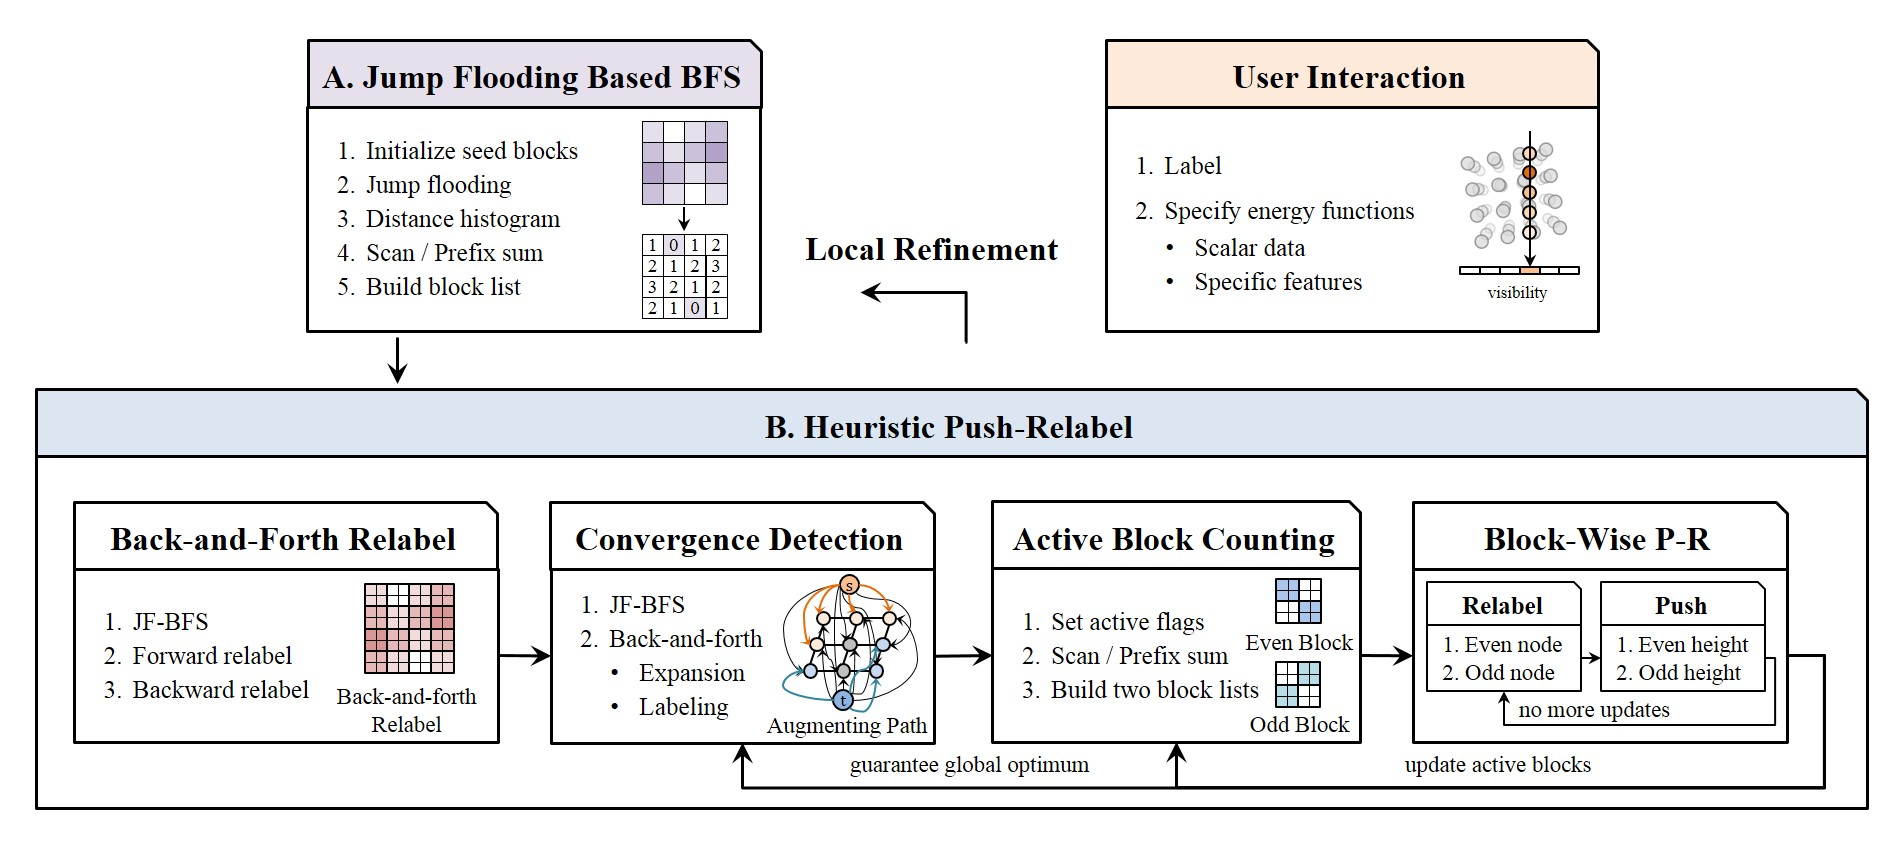
\includegraphics[width=17cm]{figures/fig1.jpg}
\caption{Our approach consists of two parts: jump flooding based BFS and heuristic push-relabel.
}
\label{figure overview}
\end{figure*}

%-------------------------------------------------------------------------
\subsection{Preliminary Knowledge}

\paragraph*{\textbf{Push-Relabel}}
starts with an excess flow (or preflow, allowing a node to have more outwards flow than inwards flow) and pushes an excess flow closer towards a sink (if the excess flow cannot reach a sink, it is pushed backwards to a source), until the maximum flow is found.
Because different active nodes (with excess flows) can be pushed or relabeled simultaneously, this algorithm has a high parallelism.
Moreover, several heuristic schemes, such as \textit{Global Relabel} and \textit{Gap Heuristics}, can be used to further improve the performance.

\paragraph*{\textbf{Global Relabel}}

computes height values (lower bound of the node's distance from the sink in the residual graph) by performing a Breadth-First Search (BFS) starting from the sink.
This heuristic technique can greatly reduce the number of iterations, because it implicitly finds out the augmenting-paths and pushes a node in the optimal direction.
This technique is used in the first stages of our approach because recomputing the height field (formed by the height of each node) in later stages is not effective and time-consuming.

\paragraph*{\textbf{Convergence Detection}}

starts from a source (or a sink) and performs a BFS on the residual network to check whether a path from a source to a sink exists:
no existence means the minimum cut is found, which partitions the graph into two parts; otherwise, the push-relabel should be continued.
Generally, the search should start from a source, because it allows us to do labeling at the same time, instead of starting from a sink and reversing its results to get the set of all neutral nodes (belonging to neither foreground, nor background) which is useless.
This technique ensures optimal results and avoids unnecessary iterations.

\paragraph*{\textbf{Jump Flooding}}

was first used to compute Voronoi Diagram (similar to Euclidean Distance Transform) for various applications in Computation Geometry and Pattern Recognition \cite{03MQR, 06RT}.
It can quickly compute the \textit{Nearest Seed Point} (NSP) of each point.
The main idea is to replace the NSP of the current point with the nearest one of the NSPs of all its neighboring points. The size of the neighborhood is halved in each iteration.
\textit{Jump Flooding} (JF) can be used to accelerate BFS in computing the nearest distance.
Given the nearest point, the nearest distance can be derived, if each neighboring point is connected with each other.
Section 3.2 gives an example of using JF to accelerate BFS.

%-------------------------------------------------------------------------
\subsection{Overview}

The key idea of our method is to accelerate the propagation of flow in the graph. We propose a convergence detection technique to ensure accuracy that is not achieved in \cite{08VN} and a block-wise push-relabel technique to achieve a faster convergence speed compared with \cite{11W}.

Our approach consists of two parts as shown in \figurename \ref{figure overview}: jump flooding based BFS and heuristic push-relabel.

Part A (jump flooding based BFS) is a basic module of our algorithm, which improves the performance of multi-pass global relabel and convergence detection.

Part B (heuristic push-relabel) is the core algorithm of our approach.
This part computes the maximum flow in an efficient way especially for large data sets, detailed in Section 3.4.
All these algorithms are parallelized with OpenCL (Open Computing Language), and evaluated with a variety of data sets.

We also design an intuitive user interface to help users specify foreground and background elements based on visibility, described in Section 4.
If the users are not satisfied with the results, they can do local refinement.

%-------------------------------------------------------------------------
\subsection{Jump Flooding Based BFS}

We use JF to accelerate Global Relabel and Convergence Detection, because both of them on the BFS.
In general, for GPU computing, the data set is often divided into blocks (each block can contain 64 to 512 threads) to fit the hardware architecture for high efficiency.
When the data set is small, using the CPU to fulfill BFS is adequate. However, when the size becomes much larger, the increasing cost should receive additional consideration.
For instance, if the data size is $1024 \times 1024 \times 512$ and the maximum block size is 256, we have to deal with nearly four million blocks.
Accordingly, we introduce a Jump Flooding based algorithm (JF-BFS), which includes five steps:

{
\small
\begin{enumerate}
\item[\textbf{F1}] Initialize all the seed blocks that contain seed nodes;
\item[\textbf{F2}] Perform jump flooding;
\item[\textbf{F3}] For each block, compute its nearest distance to the seed blocks and the distance histogram;
\item[\textbf{F4}] Perform the scan primitive on the distance histogram;
\item[\textbf{F5}] Build the block list according to the prefix sum of distance histogram.
\end{enumerate}
}

Note that, all the above steps can be performed on the GPU.
In \textbf{F1}, a seed block is defined to have at least one foreground or background node, whose \textit{Nearest Seed Block} (NSB) is initialized as itself.
Other blocks' NSBs are set to infinity.
In \textbf{F2}, we perform the standard Jump Flooding Algorithm (JFA).
In \textbf{F3}, for each block $\mathbf{p}$, we compute the distance to its NSB as the nearest distance $h$ to all the seed blocks (see Algorithm 1).
In \textbf{F4}, we compute the distance histogram and label each block a corresponding order in the bin.
In \textbf{F5}, we compute its prefix sum \cite{11MG} and calculate the final positions of all the blocks in the list.

\begin{figure}
\centering
\subfigure[Jump Size $2$]{
    \label{figure step 2}
    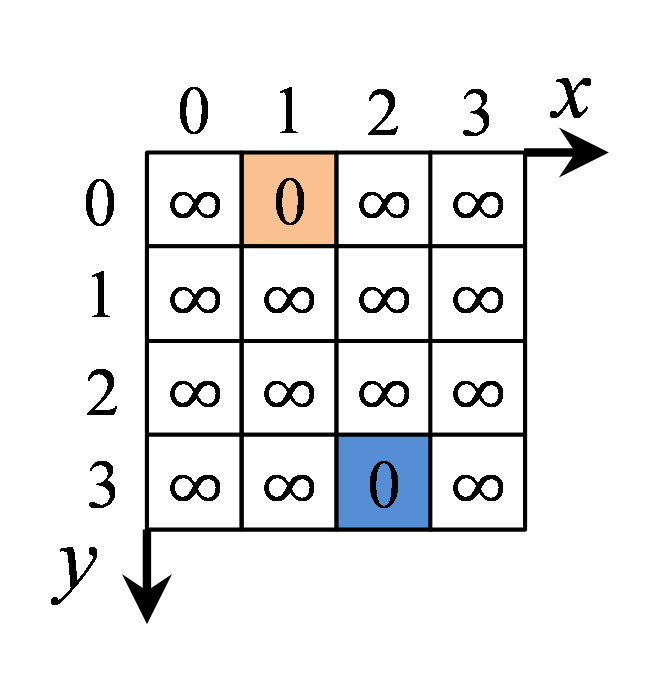
\includegraphics[width=2.55cm]{figures/fig3a.png}
    }
\subfigure[Direction $X$]{
    \label{figure step 2 x}
    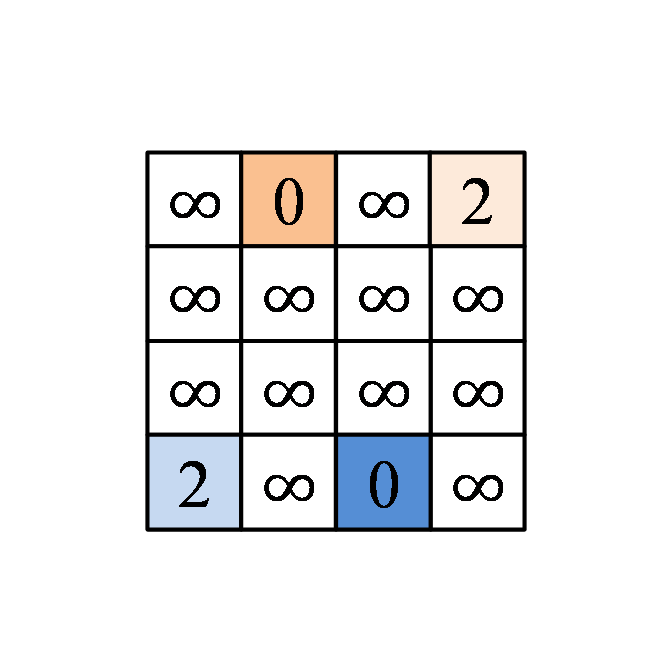
\includegraphics[width=2.55cm]{figures/fig3b.png}
    }
\subfigure[Direction $Y$]{
    \label{figure step 2 y}
    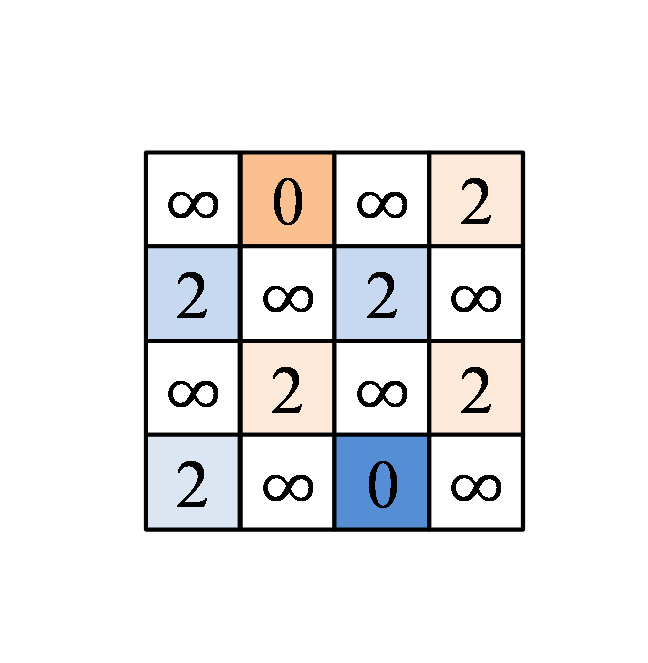
\includegraphics[width=2.55cm]{figures/fig3c.png}
    }
\\
\subfigure[Jump Size $1$]{
    \label{figure step 1}
    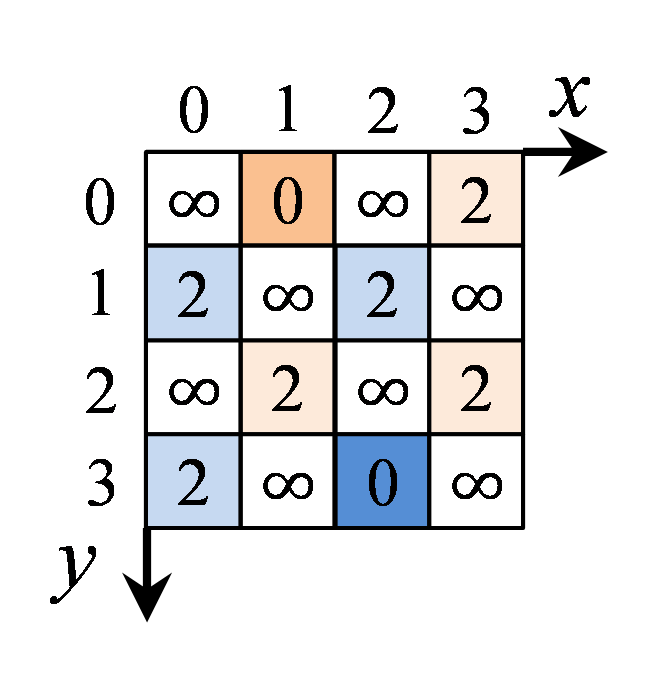
\includegraphics[width=2.55cm]{figures/fig3d.png}
    }
\subfigure[Direction $X$]{
    \label{figure step 1 x}
    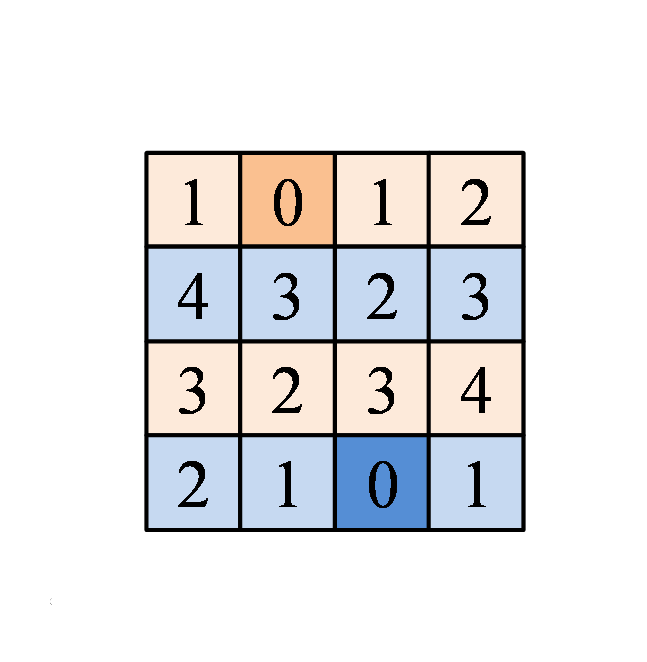
\includegraphics[width=2.55cm]{figures/fig3e.png}
    }
\subfigure[Direction $Y$]{
    \label{figure step 1 y}
    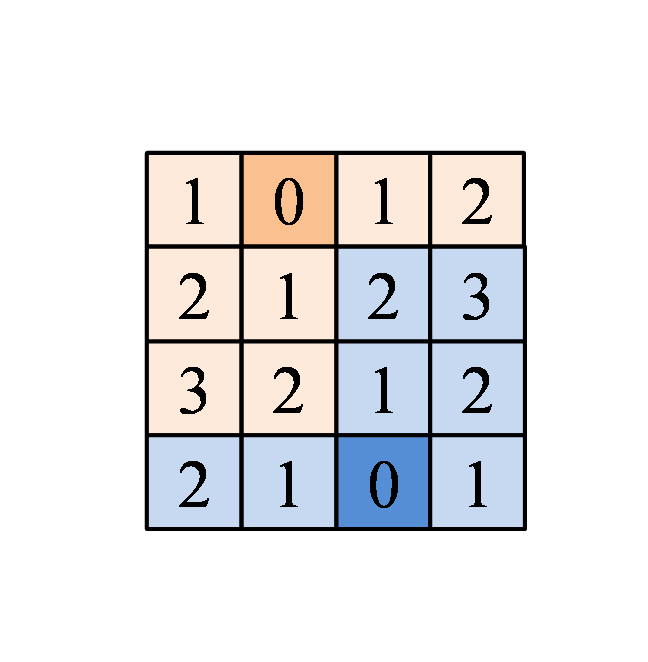
\includegraphics[width=2.55cm]{figures/fig3f.png}
    }
\caption{Jump Flooding. Two seed blocks are colored in dark orange and dark blue.
(a)-(c): the 1st flooding with $Size = 2$. Six blocks with light colors update their nearest seed blocks. Two of them are in $x$ direction and four of them are in $y$ direction.
(d)-(f): the 2nd flooding with $Size = 1$. The rest of the blocks updates the distances to their nearest seed blocks (see the integers in pixels).
}
\label{figure jump flooding}
\end{figure}

\figurename \ref{figure jump flooding} illustrates the process by taking a $4 \times 4$ network as an example.
The seed blocks are (1,0) and (2,3) and the number inside a block shows the current distance to the NSB.
In this case, the JFA includes two iterations.
The step size in the first iteration is 2 (\figurename \ref{figure step 2}-\ref{figure step 2 y}) while in the second iteration it is halved to be 1 (\figurename \ref{figure step 1}-\ref{figure step 1 y}).
In the first iteration, according to the neighbors in the $x$ direction, the NSBs of block (3, 0) and (0, 3) are updated to (1, 0) and (0, 3) respectively.
After that, block (0, 1), (2, 1), (0, 3) and (2, 3) are updated by taking the vertical neighbors into consideration.
In the second iteration, we process these blocks in the same way using a smaller step size.
Finally, eight blocks, colored in yellow have the same NSB - block (1, 0) while the other blocks, colored in blue are the nearest to block (2, 3), see \figurename \ref{figure step 1 y}.
The corresponding pseudo code is:

\begin{algorithm}
\label{algorithm jump flooding}
\caption{$\texttt{Jump Flooding}(Size, Nearest)$}
\begin{algorithmic}
\STATE $\mathbf{p} \leftarrow \texttt{Global-ID}$
\STATE $\mathbf{q} \leftarrow Nearest[x_p, y_p]$
\STATE $d \leftarrow \texttt{Taxicab-Distance} (\mathbf{p}, \mathbf{q})$
\FOR {each $\mathbf{p}_t \in \texttt{Neighbors} (\mathbf{p}, Size)$}
    \STATE $\mathbf{q}_t \leftarrow Nearest[x_{p_t}, y_{p_t}]$
    \STATE $d_t \leftarrow \texttt{Taxicab-Distance} (\mathbf{p}, \mathbf{q}_t)$
    \IF{$d_t < d$}
        \STATE $d \leftarrow d_t$
        \STATE $\mathbf{q} \leftarrow \mathbf{q}_t$
    \ENDIF
\ENDFOR
\STATE $Nearest[x_p, y_p] \leftarrow \mathbf{q}$
\end{algorithmic}
\end{algorithm}

%-------------------------------------------------------------------------
\subsection{Heuristic Push-Relabel}
\label{section hpr}

The basic idea of \textit{Heuristic Push-Relabel} is to process a block like a node, meaning that the push and relabel operations are repeated inside a block until it is saturated (no more updates for push and relabel).
Compared to the global push or relabel scheme, ours has two advantages.
First, the synchronization operations in a block can avoid data conflict for push and relabel, and local memory can be efficiently used to cache intermediate data.
Second, an alternate push and relabel improves the propagation speed of information because a node along each direction is pushed at the same time.

This scheme is more efficient than \textit{Wave Push} which only handles one direction each time.
Moreover, it allows us to take advantage of data locality and skip some of the directions.

Our method includes 4 steps:

{
\small
\begin{enumerate}
\item[\textbf{H1}] Perform JF-BFS to build the block list and perform a back-and-forth relabel;
\item[\textbf{H2}] Repeat \textbf{H3} $k_1$ times and use JF-BFS to build the list and perform the convergence detection;
    \begin{enumerate}
    \item[\textbf{H2.1}] Perform JF-BFS to build the block list starting from the foreground nodes and repeat \textbf{H2.2} until detection failed or no more nodes are marked;
    \item[\textbf{H2.2}] Perform back-and-forth detection;
        \begin{enumerate}
        \item[\textbf{H2.2.1}] If any background node is found return to \textbf{H2.1} (detection fails, keep iterating), otherwise repeat \textbf{H2.1.2} until no more nodes are marked (detection succeeds, stop iterating);
        \item[\textbf{H2.2.2}] Mark the current node as visited according to the state (visited or not) of its neighbors.
        \end{enumerate}
    \end{enumerate}
\item[\textbf{H3}] Repeat \textbf{H4} $k_2$ times, count active blocks and use Scan to build two block lists for even blocks and odd blocks;
    \begin{enumerate}
    \item[\textbf{H3.1}] For each block, set its flag as whether it contains active nodes;
    \item[\textbf{H3.2}] Perform scan primitive on the flags;
    \item[\textbf{H3.3}] Build two lists for even and odd blocks respectively;
    \end{enumerate}
\item[\textbf{H4}] Perform push-relabel for even blocks and odd blocks respectively;
    \begin{enumerate}
    \item[\textbf{H4.1}] Repeat \textbf{H4.1} until no more nodes can be pushed;
    \item[\textbf{H4.2}] Relabel even nodes and odd nodes respectively, then push them in the same way.
    \end{enumerate}
\end{enumerate}
}

%-------------------------------------------------------------------------
\subsubsection{Back-and-Forth Relabel}

In \textbf{H1}, we first use JF-BFS to build the block list for subsequent scheduling.
Based on the list, we perform a back-and-forth relabel, which processes the blocks in an ascending order and then in a descending order.
It can help us find out the paths that often change directions.
The reason is that after we finish relabel in one direction, the paths that pass along the same direction have already been found and we can easily find out all paths that change their directions only once if we try an opposite direction.
For JF-BFS, the seed blocks include background nodes (with negative excess flow).

%-------------------------------------------------------------------------
\subsubsection{Convergence Detection}

In \textbf{H2}, we detect global convergence while labeling the cutting results by checking whether there exists an augmenting-path in the residual network.
If so, we need further actions to increase the flow, otherwise we found the maximum flow.
We perform JF-BFS from the foreground nodes (source-connected) because it can mark the final results and avoid neutral nodes (see Section 3.1).

The principle implied by these sub-steps is that when we get the maximum flow(or minimum cut), the residual network will be divided into two parts, and for each part all nodes should be connected, and all edges belonging to the minimum cut should be saturated.
It indicates that we can start from one part and repeat expanding nodes to decide whether we have found the global optimum.

This step ensures that our algorithm can find the maximum flow and get the optimal results.
In our implementation, due to the expensive cost of this procedure, we repeat \textbf{H3} $k_1$ times and perform it once.
$k_1$ defaults to 4 (performs best for median-size image) and can be specified by users.
Generally, it would be better to increase $k_1$ when the data size increases (16 is better for large images and videos).

%-------------------------------------------------------------------------
\subsubsection{Active Block Counting}

Active Block Counting is designed to reduce the computational cost by building a block list for active blocks, which is mainly based on the two facts: during the process only some nodes can be pushed or relabeled, and the number of active nodes decreases when more data is processed.
So only process active nodes efficiently improve the performance.
Because active-blocks change slowly, we can do one counting after $k_2$ iterations.
$k_2$ is set to be 4 (better for median-size data sets) and is user-adjustable.
This procedure includes three sub-steps (see \textbf{H3.1}~\textbf{H3.3}).
We use two flags to record the detection results.
If the current block contains active nodes, we set its corresponding flag (even flag corresponds to even block) to be 1, otherwise 0.
After that, we perform a scan to compact the flags into a scheduling list.

%-------------------------------------------------------------------------
\subsubsection{Block-Wise Push-Relabel}

\begin{figure}
\centering
\subfigure[Wave Push]{
    \label{figure wave push}
    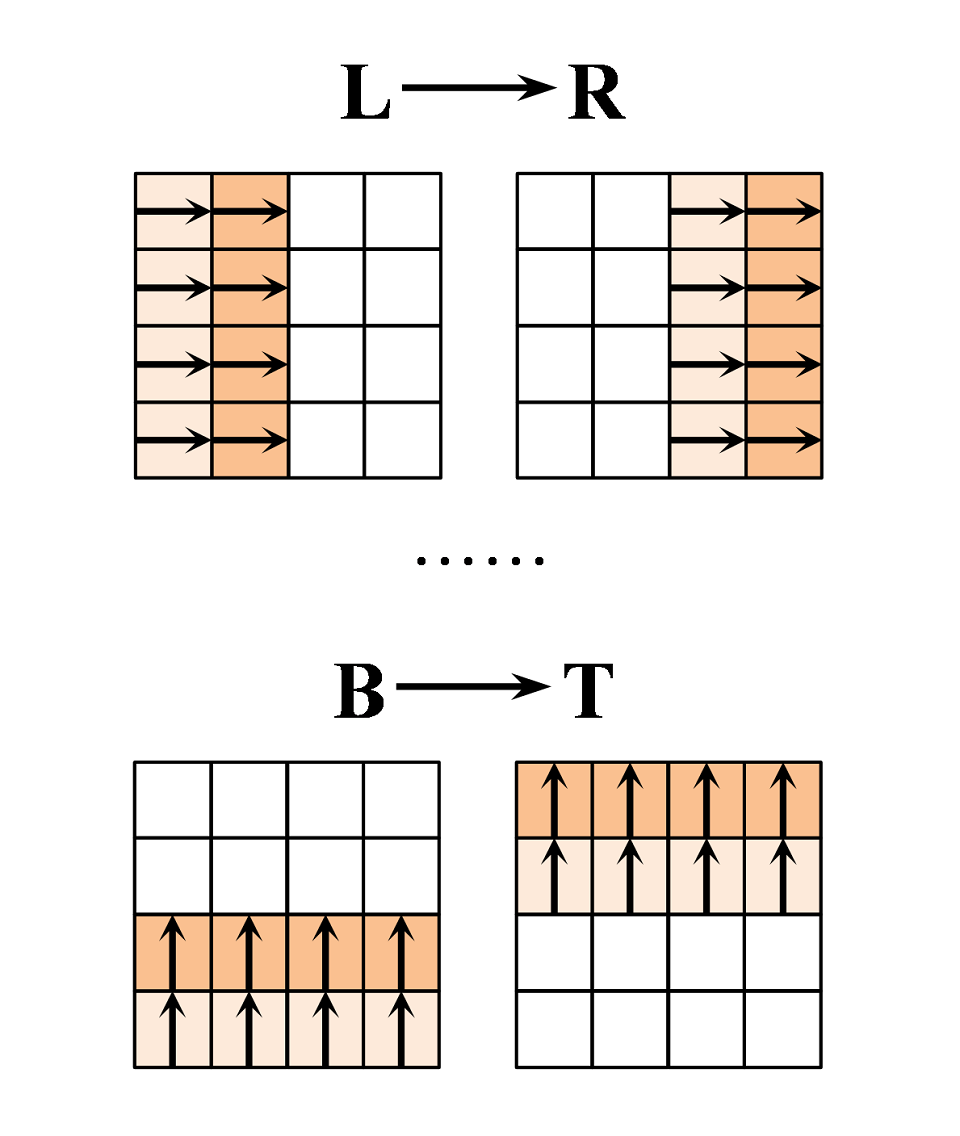
\includegraphics[width=3.5cm]{figures/fig4a.png}
    }
\subfigure[Block-Wise Push]{
    \label{figure block-wise push}
    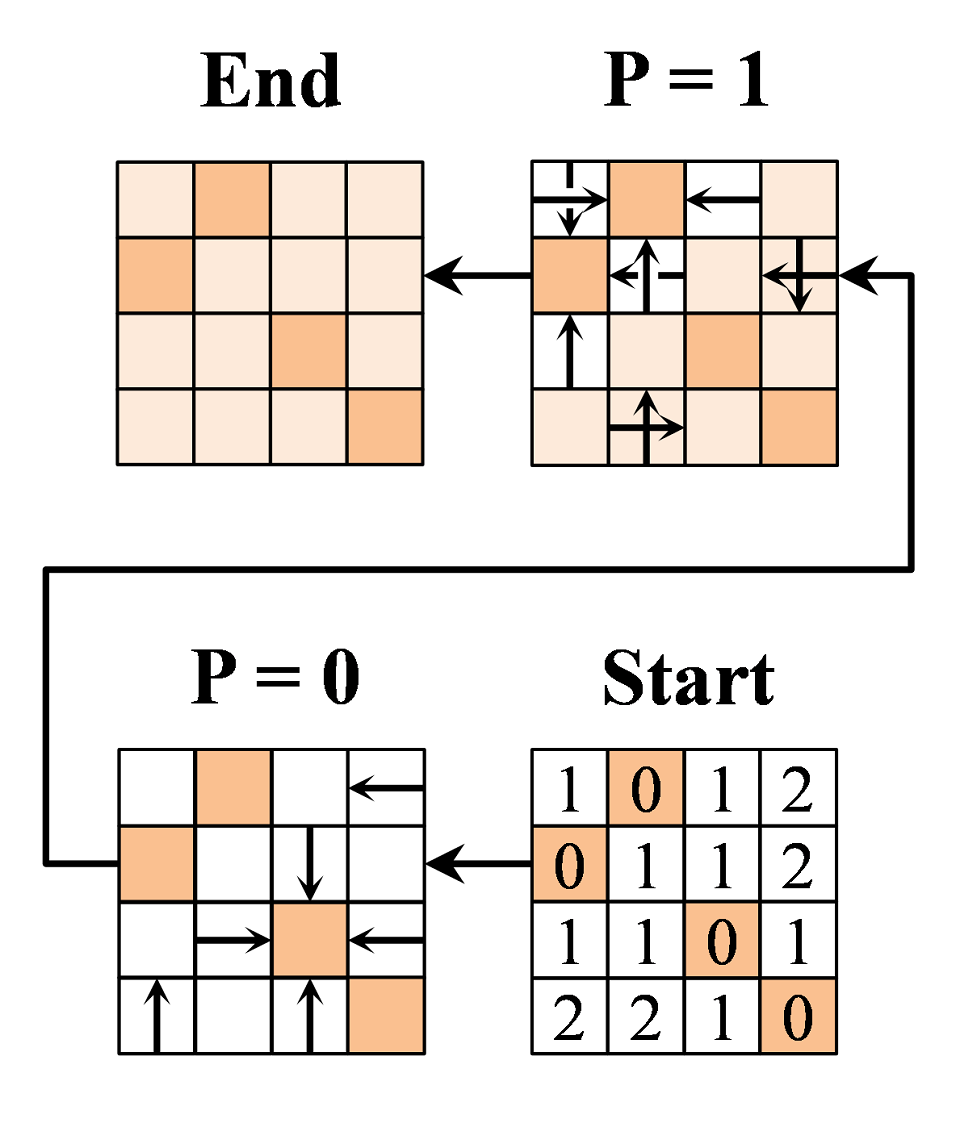
\includegraphics[width=3.5cm]{figures/fig4b.png}
    }
\caption{Heuristic Push.
(a): only handles one direction each time.
(b): skip some directions which needn't to be processed. $P$ denotes block parity.
}
\label{figure heuristic push}
\end{figure}

As mentioned earlier, iterative push-relabel operations inside a block takes advantage of locality and increases the propagation speed of flow compared with \textit{Wave Push} as shown in \figurename \ref{figure heuristic push}.

\begin{algorithm}
\label{algorithm block-wise p-r}
\caption{$\texttt{Push-Relabel}(Node)$}
\begin{algorithmic}
\STATE $\mathbf{p} \leftarrow \texttt{Local-ID}$
\STATE copy global $Node$ to local $Node'$
\STATE $d' \leftarrow false$
\STATE \texttt{barrier()}
\WHILE {\NOT $d'$}
    \STATE $t_a \leftarrow \texttt{Active}(Node'[x_p, y_p])$
    \STATE $t_p \leftarrow (x_p + y_p)$ mod $2$
    \IF{$t_a$ \AND $t_p = 0$}
       \STATE $ \texttt{Relabel}()$
    \ENDIF
    \STATE \texttt{barrier()}
    \IF{$t_a$ \AND $t_p = 1$}
       \STATE $ \texttt{Relabel}()$
    \ENDIF
    \STATE $d' \leftarrow true$
    \STATE \texttt{barrier()}

    \STATE $t_a \leftarrow \texttt{Active}(Node'[x_p, y_p])$
    \IF{$t_a$ \AND $t_p = 0$ \AND $\texttt{Push}()$}
        \STATE $d' \leftarrow false$
    \ENDIF
    \STATE \texttt{barrier()}
    \IF{$t_a$ \AND $t_p = 1$ \AND $\texttt{Push}()$}
        \STATE $d' \leftarrow false$
    \ENDIF
    \STATE \texttt{barrier()}
\ENDWHILE
\STATE copy local $Node'$ to global $Node$
\end{algorithmic}
\end{algorithm}

The kernel code (2D-version) is shown in Algorithm 2.
We first load the data from global memory to local memory, then perform iterative push-relabel, and finally write back the data.
In each iteration, there are two stages: relabel and push.
In the relabel stage, we first check whether $Node'[x_p, y_p]$ is active, and then process even nodes with $(x_p + y_p) \, mod \, 2 = 0$ and odd nodes with $(x_p + y_p) \, mod \, 2 = 1$ respectively, because these two kinds of nodes have data conflict with each other.
In the push stage, we process the nodes in the same way.
Both directions are handled one after another.
When a node becomes inactive after being pushed in one direction, we skip the following directions.
In this way, many unnecessary computations can be avoided.
Then we process the nodes in the same way.



%-------------------------------------------------------------------------
\section{User Interaction}
\label{section user interaction}

We design a user interface for both images and videos.
It helps users mark foreground and background based on visibility, build an energy function according to the scenario, make local refinements and finally shows the graph cut results.

%-------------------------------------------------------------------------
\subsection{Labeling}

For videos, it is quite difficult for users to specify the foreground and background elements.
The conventional way is to mark the nodes frame by frame, which is time-consuming.
In our system, we provide users a WYSIWYG way to do labeling (both for images and videos).
The basic idea is to mark what users actually see based on visibility.
This technique is combined with a ray casting algorithm which requires users to specify a visibility threshold \cite{05BS, 11CM}.

%-------------------------------------------------------------------------
\subsection{Scenario-Driven Energy Function}

An \textit{Energy Function} is used to define the capacity of each edge in the graph, which measures the similarity of different subsets.
The generic form of the energy function is given by:

\begin{equation}
\label{equation energy function}
E = \lambda \sum R(p) + \sum B(p, q)
\end{equation}

where $R$ and $B$ denote the region properties and boundary properties respectively, $\lambda$ specifies a relative importance of the region properties versus the boundary properties.
We provide users with different ways to build the energy function for different scenarios.

\paragraph*{\textbf{Scalar Field Data}} we simplify the energy function introduced by Boykov-Kolmogorov \cite{04BK} which uses a probability distribution to measure the similarity and has a low accuracy.
We propose to focus on the continuity of a structure:

\begin{equation}
\label{equation bk_capacity}
C_{s}(p,q) = \left\{
    \begin{array}{ll}
    0 & p, q \in \mathcal{F} \bigcup \mathcal{B}\\
    exp(-\frac{(I_p - I_q)^2}{2\sigma^2}) & otherwise
    \end{array}
\right.
\end{equation}

\begin{equation}
\label{equation bk_excessflow}
E_{s}(p) = \left\{
    \begin{array}{ll}
    +E_{max} & p \in \mathcal{F}\\
    -E_{max} & p \in \mathcal{B}\\
    0 & p \in \mathcal{U}
    \end{array}
\right.
\end{equation}

where the nodes are divided into three groups: $\mathcal{F}$(foreground), $\mathcal{B}$(background) and $\mathcal{U}$(unknown).
$C_s$ denotes the capacity of the neighboring edge, $E_s$ denotes the excess flow of a node.
$I$ denotes the intensity and $\sigma$ can be estimated as "sampling error".

\paragraph*{\textbf{Vector Field Data}} We define the region and boundary terms similar to \textit{Lazy Snapping} which measures the similarity in the feature-space:

\begin{equation}
\label{equation lazy capacity}
C_{v}(p,q) = \left\{
    \begin{array}{ll}
    0 & p, q \in \mathcal{F} \bigcup \mathcal{B}\\
    \frac{1}{1 + \| \mathbf{v}_p - \mathbf{v}_q \|} & otherwise
    \end{array}
\right.
\end{equation}

\begin{equation}
\label{equation lazy excessflow}
E_{v}(p) = \left\{
    \begin{array}{ll}
    +E_{max} & p \in \mathcal{F}\\
    -E_{max} & p \in \mathcal{B}\\
    \lambda \frac{\min{\|\mathbf{c}_i^\mathcal{B}-\mathbf{v}_p \|} - \min{\|\mathbf{c}_i^\mathcal{F}-\mathbf{v}_p \|}}{\min{\|\mathbf{c}_i^\mathcal{B}-\mathbf{v}_p \|} + \min{\|\mathbf{c}_i^\mathcal{F}-\mathbf{v}_p \|}} & p \in \mathcal{U}
    \end{array}
\right.
\end{equation}

where $C_v$ denotes the neighbor-capacity, $E_v$ denotes the excess flow and is defined by the minimum distance to the center of a cluster which the current node belongs to.
These centers are computed by \textit{K-Means Clustering} which is also parallelized.
It helps us extract key features from the foreground and background, so that the noises can be effectively restrained and the accuracy is improved.
In this algorithm, the number of clusters $k$ is set to be 8, and the seed points are initialized using a histogram equalization technique.

Our system also supports features extraction, which can convert a scalar data into a multi-dimensional data \cite{10PC}.
These features include gradient, hessian matrix \cite{02KKH} and curvature \cite{03KWTM}.



%-------------------------------------------------------------------------
\section{Results}
\label{section results}

We implement an integrated system using OpenCL 1.0 and QT 4.8.
Our system supports across heterogeneous platforms.
The experimental environment is: Windows 8 64bit with Intel (R) Core i7-3770 @ 3.40GHz and NVIDIA GeForce GTX TITAN @ 6GB (or AMD Radeon HD 7990 @ 2$\times$3GB).
Different kinds of data sets are used to evaluate our method, and we compare our algorithm with both CPU based methods and GPU based methods.

%-------------------------------------------------------------------------
\subsection{Datasets}

We tested two kinds of data sets.
One of them is a part of the benchmark provided by Grid-Cut \cite{12JSH}.
The other is downloaded from the Internet, which includes high-resolution images, HD videos and volume data sets.
Below is the detail information of the data sets and the scaled-up versions of the data sets.
The performance of different algorithms is summarized in \tablename \ \ref{table benchmark}.

\begin{table}
\center
\caption{Benchmark Datasets}
\label{table benchmark}
{
    \fontsize{6.5pt}{8pt}\selectfont
    \begin{tabular}{@{ }c|r|r@{ }r@{ }r|r|c@{ }}
    \hline\rule{0pt}{0.3cm}
    Name & Scale & Width & Height & Depth & Max Flow & Size (MB)\\
    \hline\rule{0pt}{0.30cm}
       \multirow{3}{*}{\specialcell{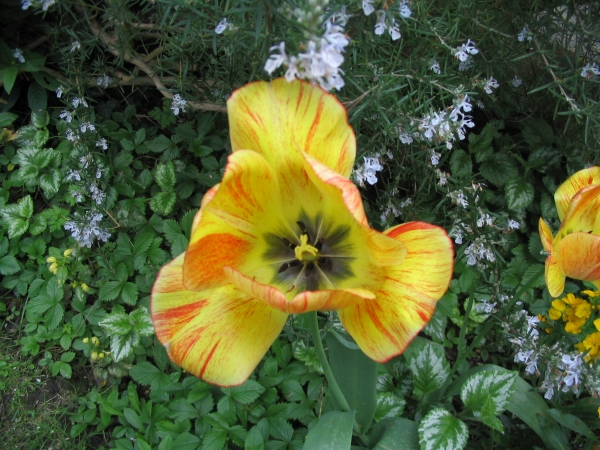
\includegraphics[width=0.70cm]{figures/fig5a.png}\\Flower(M)}}
       & 1 x 1     & 600   & 450   & 1     & 1208089    & 3.35\\
       & 4 x 4     & 2400  & 1800  & 1     & 7856011    & 53.5\\
       & 16 x 16   & 9600  & 7200  & 1     & 50618597   & 856 \\
    \hline\rule{0pt}{0.30cm}
       \multirow{3}{*}{\specialcell{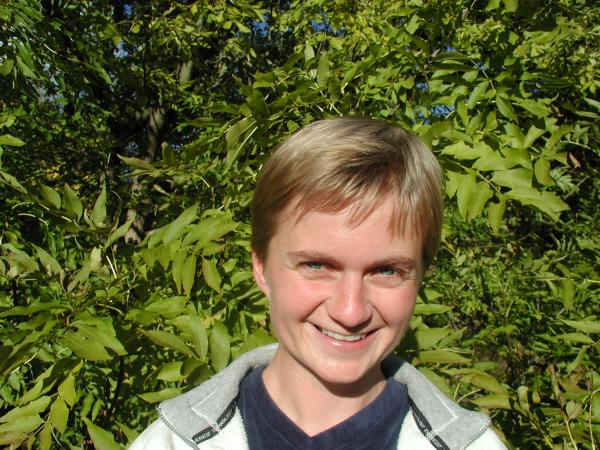
\includegraphics[width=0.70cm]{figures/fig5b.png}\\Person(M)}}
       & 1 x 1     & 600   & 450   & 1     & 880461     & 3.35\\
       & 4 x 4     & 2400  & 1800  & 1     & 5042635    & 53.5\\
       & 16 x 16   & 9600  & 7200  & 1     & 29042350   & 856 \\
    \hline\rule{0pt}{0.30cm}
       \multirow{3}{*}{\specialcell{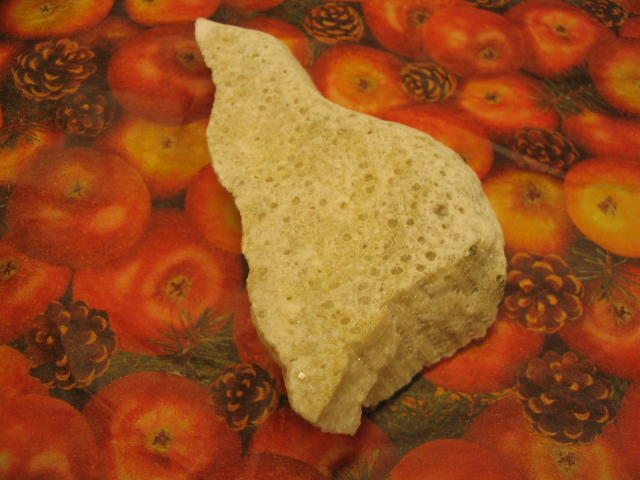
\includegraphics[width=0.70cm]{figures/fig5c.png}\\Sponge(M)}}
       & 1 x 1     & 640   & 480   & 1     & 343591     & 3.81\\
       & 4 x 4     & 2560  & 1920  & 1     & 1910718    & 60.9\\
       & 16 x 16   & 10240 & 7680  & 1     & 10136071   & 975 \\
    \hline\rule{0pt}{0.30cm}
       \multirow{3}{*}{\specialcell{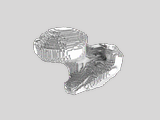
\includegraphics[width=0.70cm]{figures/fig5d.png}\\Bone(U)}}
       & 1 x 1 x 1 & 256   & 256   & 119   & 71344      & 111 \\
       & 2 x 2 x 2 & 512   & 512   & 238   & 1913780    & 892 \\
       &           &       &       &       &            &     \\
    \hline\rule{0pt}{0.30cm}
       \multirow{3}{*}{\specialcell{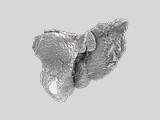
\includegraphics[width=0.70cm]{figures/fig5e.png}\\Liver(U)}}
       & 1 x 1 x 1 & 170   & 170   & 144   & 625447     & 59.5\\
       & 2 x 2 x 2 & 340   & 340   & 288   & 3886049    & 476 \\
       &           &       &       &       &            &     \\
    \hline\rule{0pt}{0.30cm}
       \multirow{3}{*}{\specialcell{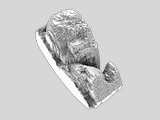
\includegraphics[width=0.70cm]{figures/fig5f.png}\\Babyface(U)}}
       & 1 x 1 x 1 & 250   & 250   & 81    & 222943     & 72.4\\
       & 2 x 2 x 2 & 500   & 500   & 162   & 3316927    & 579 \\
       &           &       &       &       &            &     \\
    \hline\rule{0pt}{0.30cm}
       \multirow{3}{*}{\specialcell{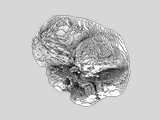
\includegraphics[width=0.70cm]{figures/fig5g.png}\\Adhead(U)}}
       & 1 x 1 x 1 & 256   & 256   & 192   & 589368     & 180 \\
       & 2 x 2 x 2 & 512   & 512   & 384   & 3594110    & 1440\\
       &           &       &       &       &            &     \\
    \hline\rule{0pt}{0.30cm}
       \multirow{3}{*}{\specialcell{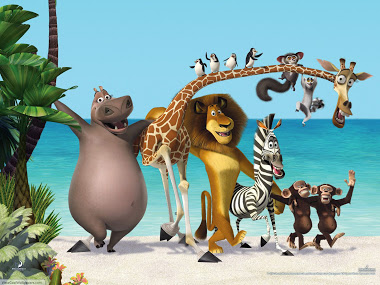
\includegraphics[width=0.70cm]{figures/fig5h.jpg}\\Madagascar(G)}}
       &           &       &       &       &            &      \\
       & 1 x 1 x 1 & 10800 & 8100  & 1     & 4946409834 & 1413 \\
       &           &       &       &       &            &      \\
    \hline\rule{0pt}{0.30cm}
       \multirow{3}{*}{\specialcell{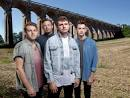
\includegraphics[width=0.70cm]{figures/fig5i.jpg}\\LTA(G)}}
       &           &       &       &       &            &      \\
       & 1 x 1 x 1 & 9900  & 7500  & 1     & 6244836523 & 1198 \\
       &           &       &       &       &            &      \\
    \hline\rule{0pt}{0.30cm}
       \multirow{2}{*}{\specialcell{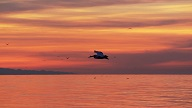
\includegraphics[width=0.70cm]{figures/fig5j.jpg}\\TimeScapes(Y)}}
       &           &       &       &       &            &      \\
       & 1 x 1 x 1 & 2560  & 1440  & 30    & 80886496   & 1577 \\
       &           &       &       &       &            &      \\
    \hline\rule{0pt}{0.30cm}
       \multirow{2}{*}{\specialcell{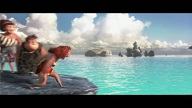
\includegraphics[width=0.70cm]{figures/fig5k.jpg}\\The Croods(Y)}}
       &           &       &       &       &            &      \\
       & 1 x 1 x 1 & 1920  & 1080  & 40    & 180301245  & 1178 \\
       &           &       &       &       &            &      \\
    \hline\rule{0pt}{0.30cm}
       \multirow{2}{*}{\specialcell{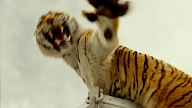
\includegraphics[width=0.70cm]{figures/fig5l.jpg}\\Life of PI(Y)}}
       &           &       &       &       &            &      \\
       & 1 x 1 x 1 & 1920  & 1080  & 32    & 1178329527 & 949  \\
       &           &       &       &       &            &      \\
    \hline\rule{0pt}{0.30cm}
       \multirow{3}{*}{\specialcell{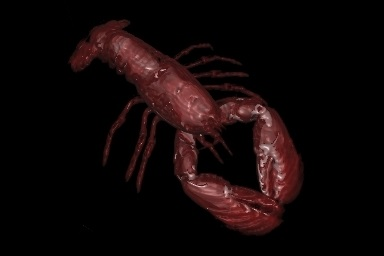
\includegraphics[width=0.70cm]{figures/fig5m.jpg}\\MRBrain(V)}}
       &           &       &       &       &            &      \\
       & 1 x 1 x 1 & 256   & 256   & 109   & 29036      & 102  \\
       &           &       &       &       &            &      \\
    \hline\rule{0pt}{0.30cm}
       \multirow{3}{*}{\specialcell{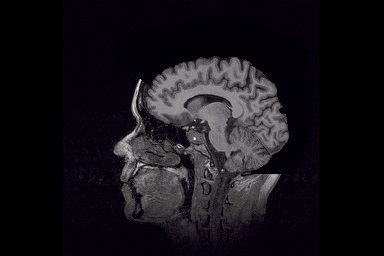
\includegraphics[width=0.70cm]{figures/fig5n.jpg}\\Lobster(V)}}
       &           &       &       &       &            &      \\
       & 1 x 1 x 1 & 301   & 324   & 56    & 238402     & 78   \\
       &           &       &       &       &            &      \\
    \hline\rule{0pt}{0.30cm}
    \end{tabular}
    \begin{tablenotes}
        \item {
        \begin{enumerate}
            \item M - Middlebury College: \url{http://vision.middlebury.edu/MRF/}
            \item U - University of Western Ontario: \url{http://vision.csd.uwo.ca/data/maxflow/}
            \item G - Google Advanced Image Search: \url{http://images.google.com/advanced_image_search}
            \item Y - YouTube: \url{http://www.youtube.com/}
            \item V - VolVis: \url{http://www.volvis.org/}
        \end{enumerate}}
    \end{tablenotes}
}
\end{table}

We conduct experiments on these large data sets to show the practicality and efficiency of our method.
In these experiments, the foreground and background are colored in magenta and green respectively, and the cut results are highlighted in yellow.

\paragraph*{\textbf{Image Segmentation}} The results include two parts, as shown in \figurename \ref{figure image segmentation}.
The first part contains standard data sets (from Middlebury) with providing energy function.
The
\textit{Lower Than Atlantis}
\footnotemark[1]\footnotetext[1]{\scriptsize Lower Than Atlantis: \url{http://fashionsoundtrack.com/wp-content/uploads/2013/08/A1posterLTA.jpg}} and
\textit{Madagascar}
\footnotemark[2]\footnotetext[2]{\scriptsize Madagascar: \url{http://wallpaper.imgcandy.com/images/233316-jessica-alba-wardrobe-malfunction-original-source-of-image.jpg}}
data sets in the second part are much larger and we use the clustering based model to set up energy function.

\begin{figure*}
\centering
\subfigure[Flower - $600 \times 450$]{
    \label{figure flower}
    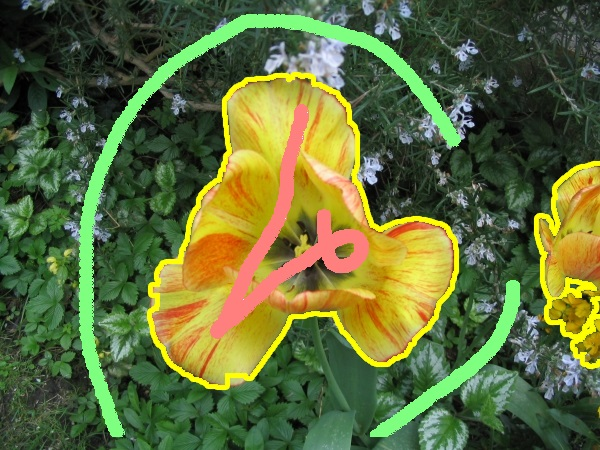
\includegraphics[width=5cm]{figures/fig7a.jpg}
    }
\subfigure[Person - $600 \times 450$]{
    \label{figure person}
    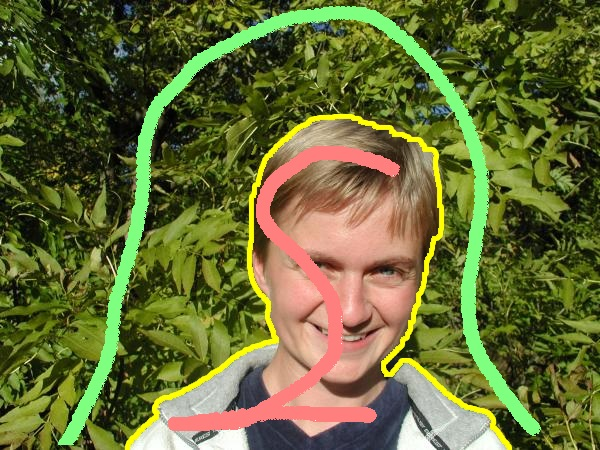
\includegraphics[width=5cm]{figures/fig7b.jpg}
    }
\subfigure[Sponge - $640 \times 480$]{
    \label{figure sponge}
    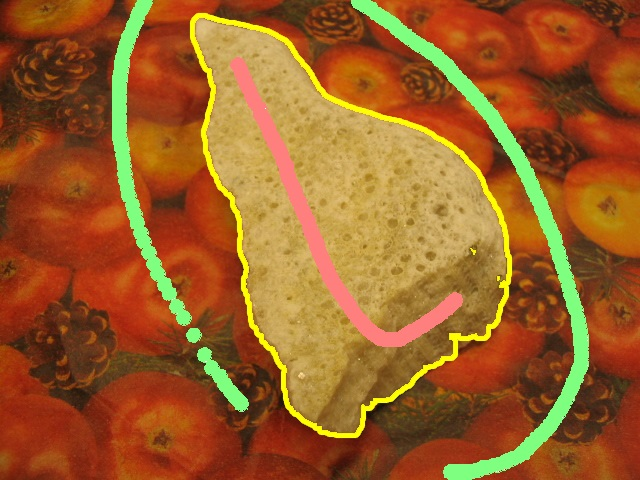
\includegraphics[width=5cm]{figures/fig7c.jpg}
    }
\\
\subfigure[Madagascar - $10800 \times 8100$]{
    \label{figure madagascar}
    \includegraphics[width=8.04cm]{figures/fig8c.jpg}
    }
\subfigure[Lower Than Atlantis - $9900 \times 7500$]{
    \label{figure lower than atlantis}
    \includegraphics[width=7.96cm]{figures/fig8d.jpg}
    }
\caption{Image Segmentation Results.
\ref{figure flower}-\ref{figure sponge}: benchmark data sets with small size.
\ref{figure lower than atlantis}-\ref{figure madagascar}: large images. \protect\footnotemark[1] \protect\footnotemark[2]
}
\label{figure image segmentation}
\end{figure*}

\paragraph*{\textbf{Video Cutout}} We use the clustering based model to build energy function.
These videos are clipped from official trailers of different films such as \textit{THE CROODS}
\footnotemark[3]\footnotetext[3]{\scriptsize TimeScapes - Trailer 2 4k 2560p: \url{http://red.cachefly.net/TimeScapes4K2560p.mp4}},
\textit{TimeScapes}
\footnotemark[4]\footnotetext[4]{\scriptsize THE CROODS - Official Trailer 3: \url{http://www.youtube.com/watch?v=xrbwgn_kRBo}} and
\textit{Life of Pi}
\footnotemark[5]\footnotetext[5]{\scriptsize Life of Pi - Trailer 2 Official: \url{http://www.youtube.com/watch?v=m7WBfntqUoA}}.
\figurename \ref{figure video cutout} shows the cutout results.

\begin{figure*}
\centering
\subfigure[TimeScapes - $2560 \times 1440 \times 30$]{
    \label{figure 4k 3d}
    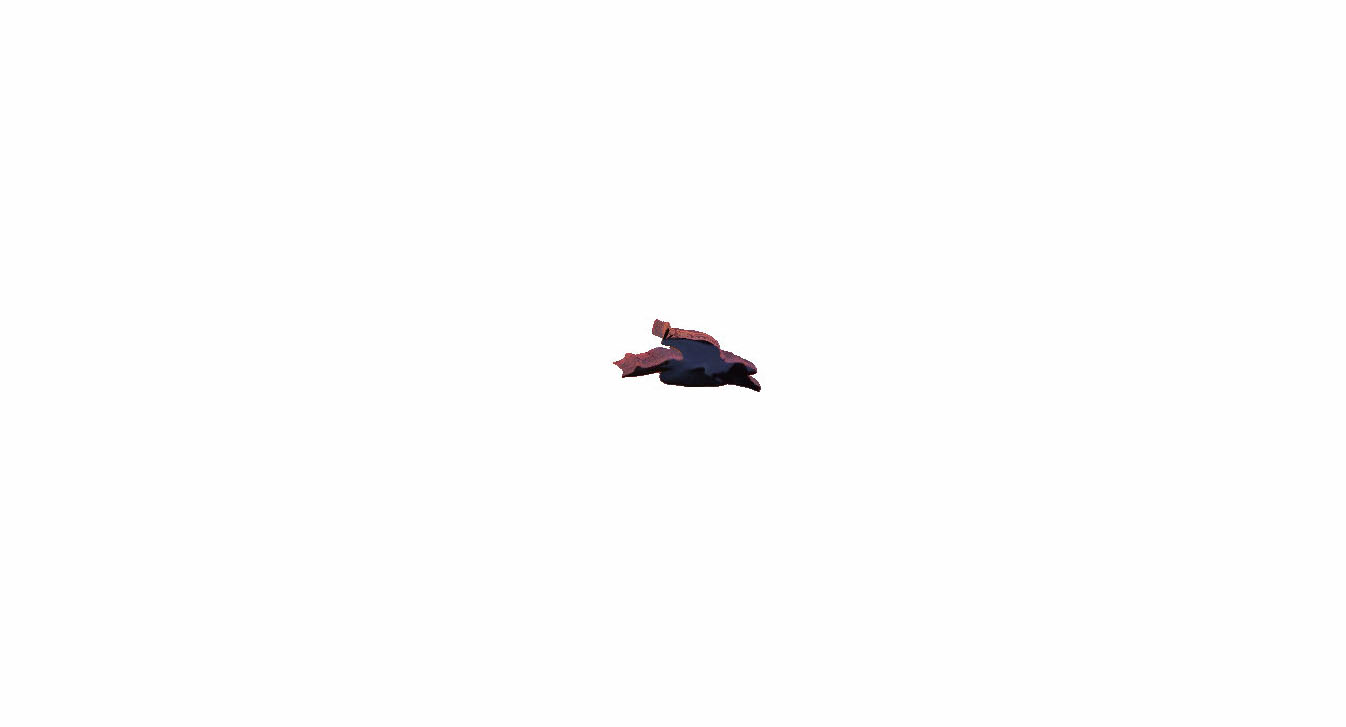
\includegraphics[width=5cm]{figures/fig16c.jpg}
    }
\subfigure[THE CROODS - $1920 \times 1080 \times 40$]{
    \label{figure eep 3d}
    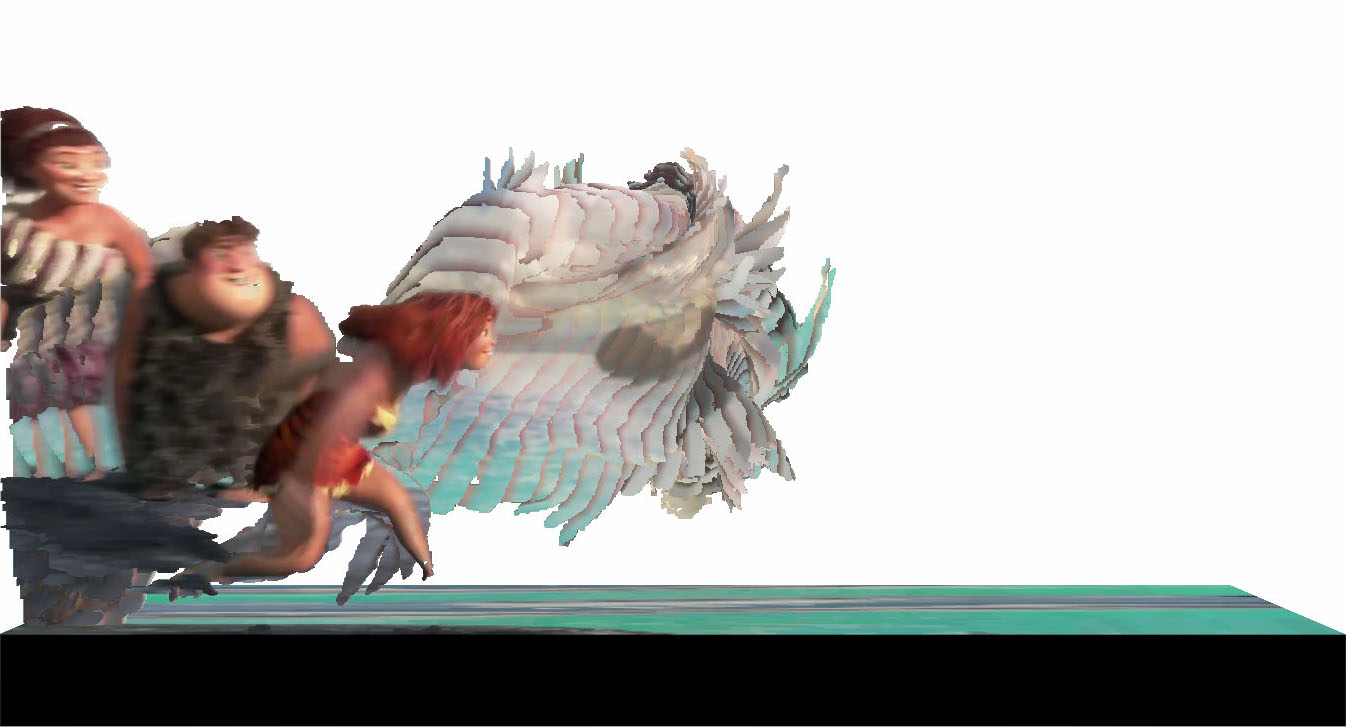
\includegraphics[width=5cm]{figures/fig14c.jpg}
    }
\subfigure[Life of PI - $1920 \times 1080 \times 36$]{
    \label{figure pi 3d}
    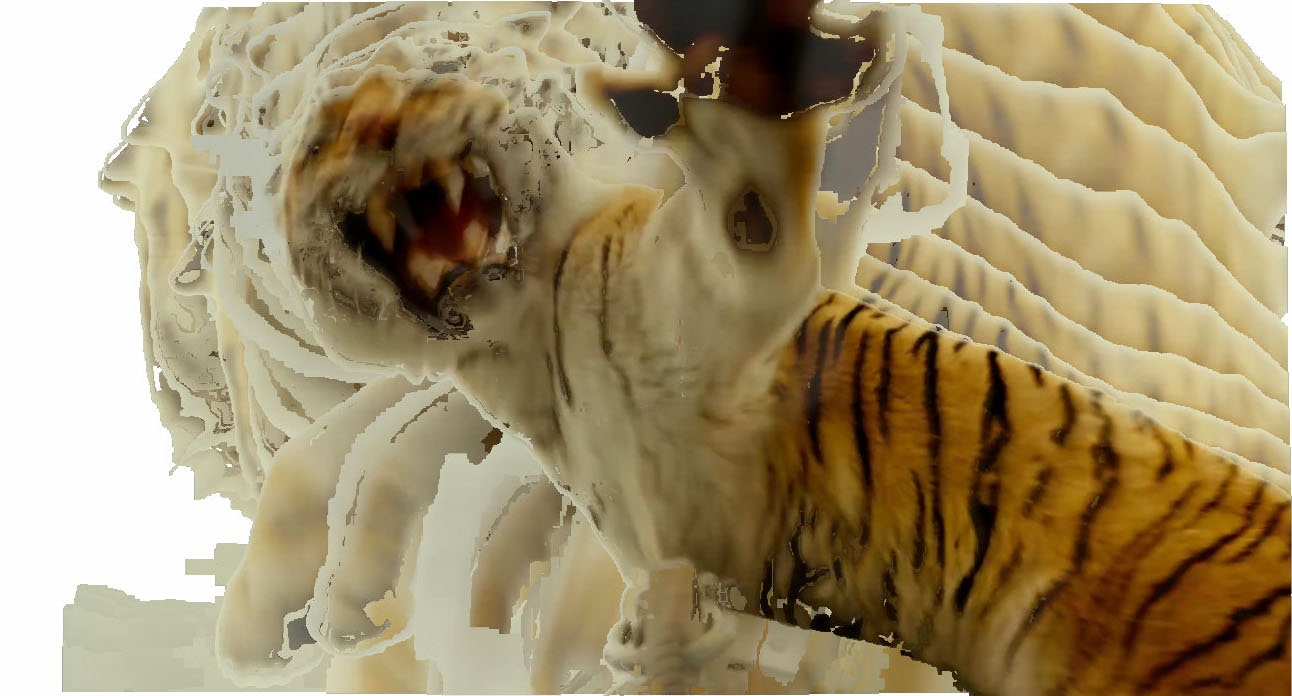
\includegraphics[width=5cm]{figures/fig15c.jpg}
    }
\\
\subfigure[TimeScapes - Frame]{
    \label{figure 4k frame}
    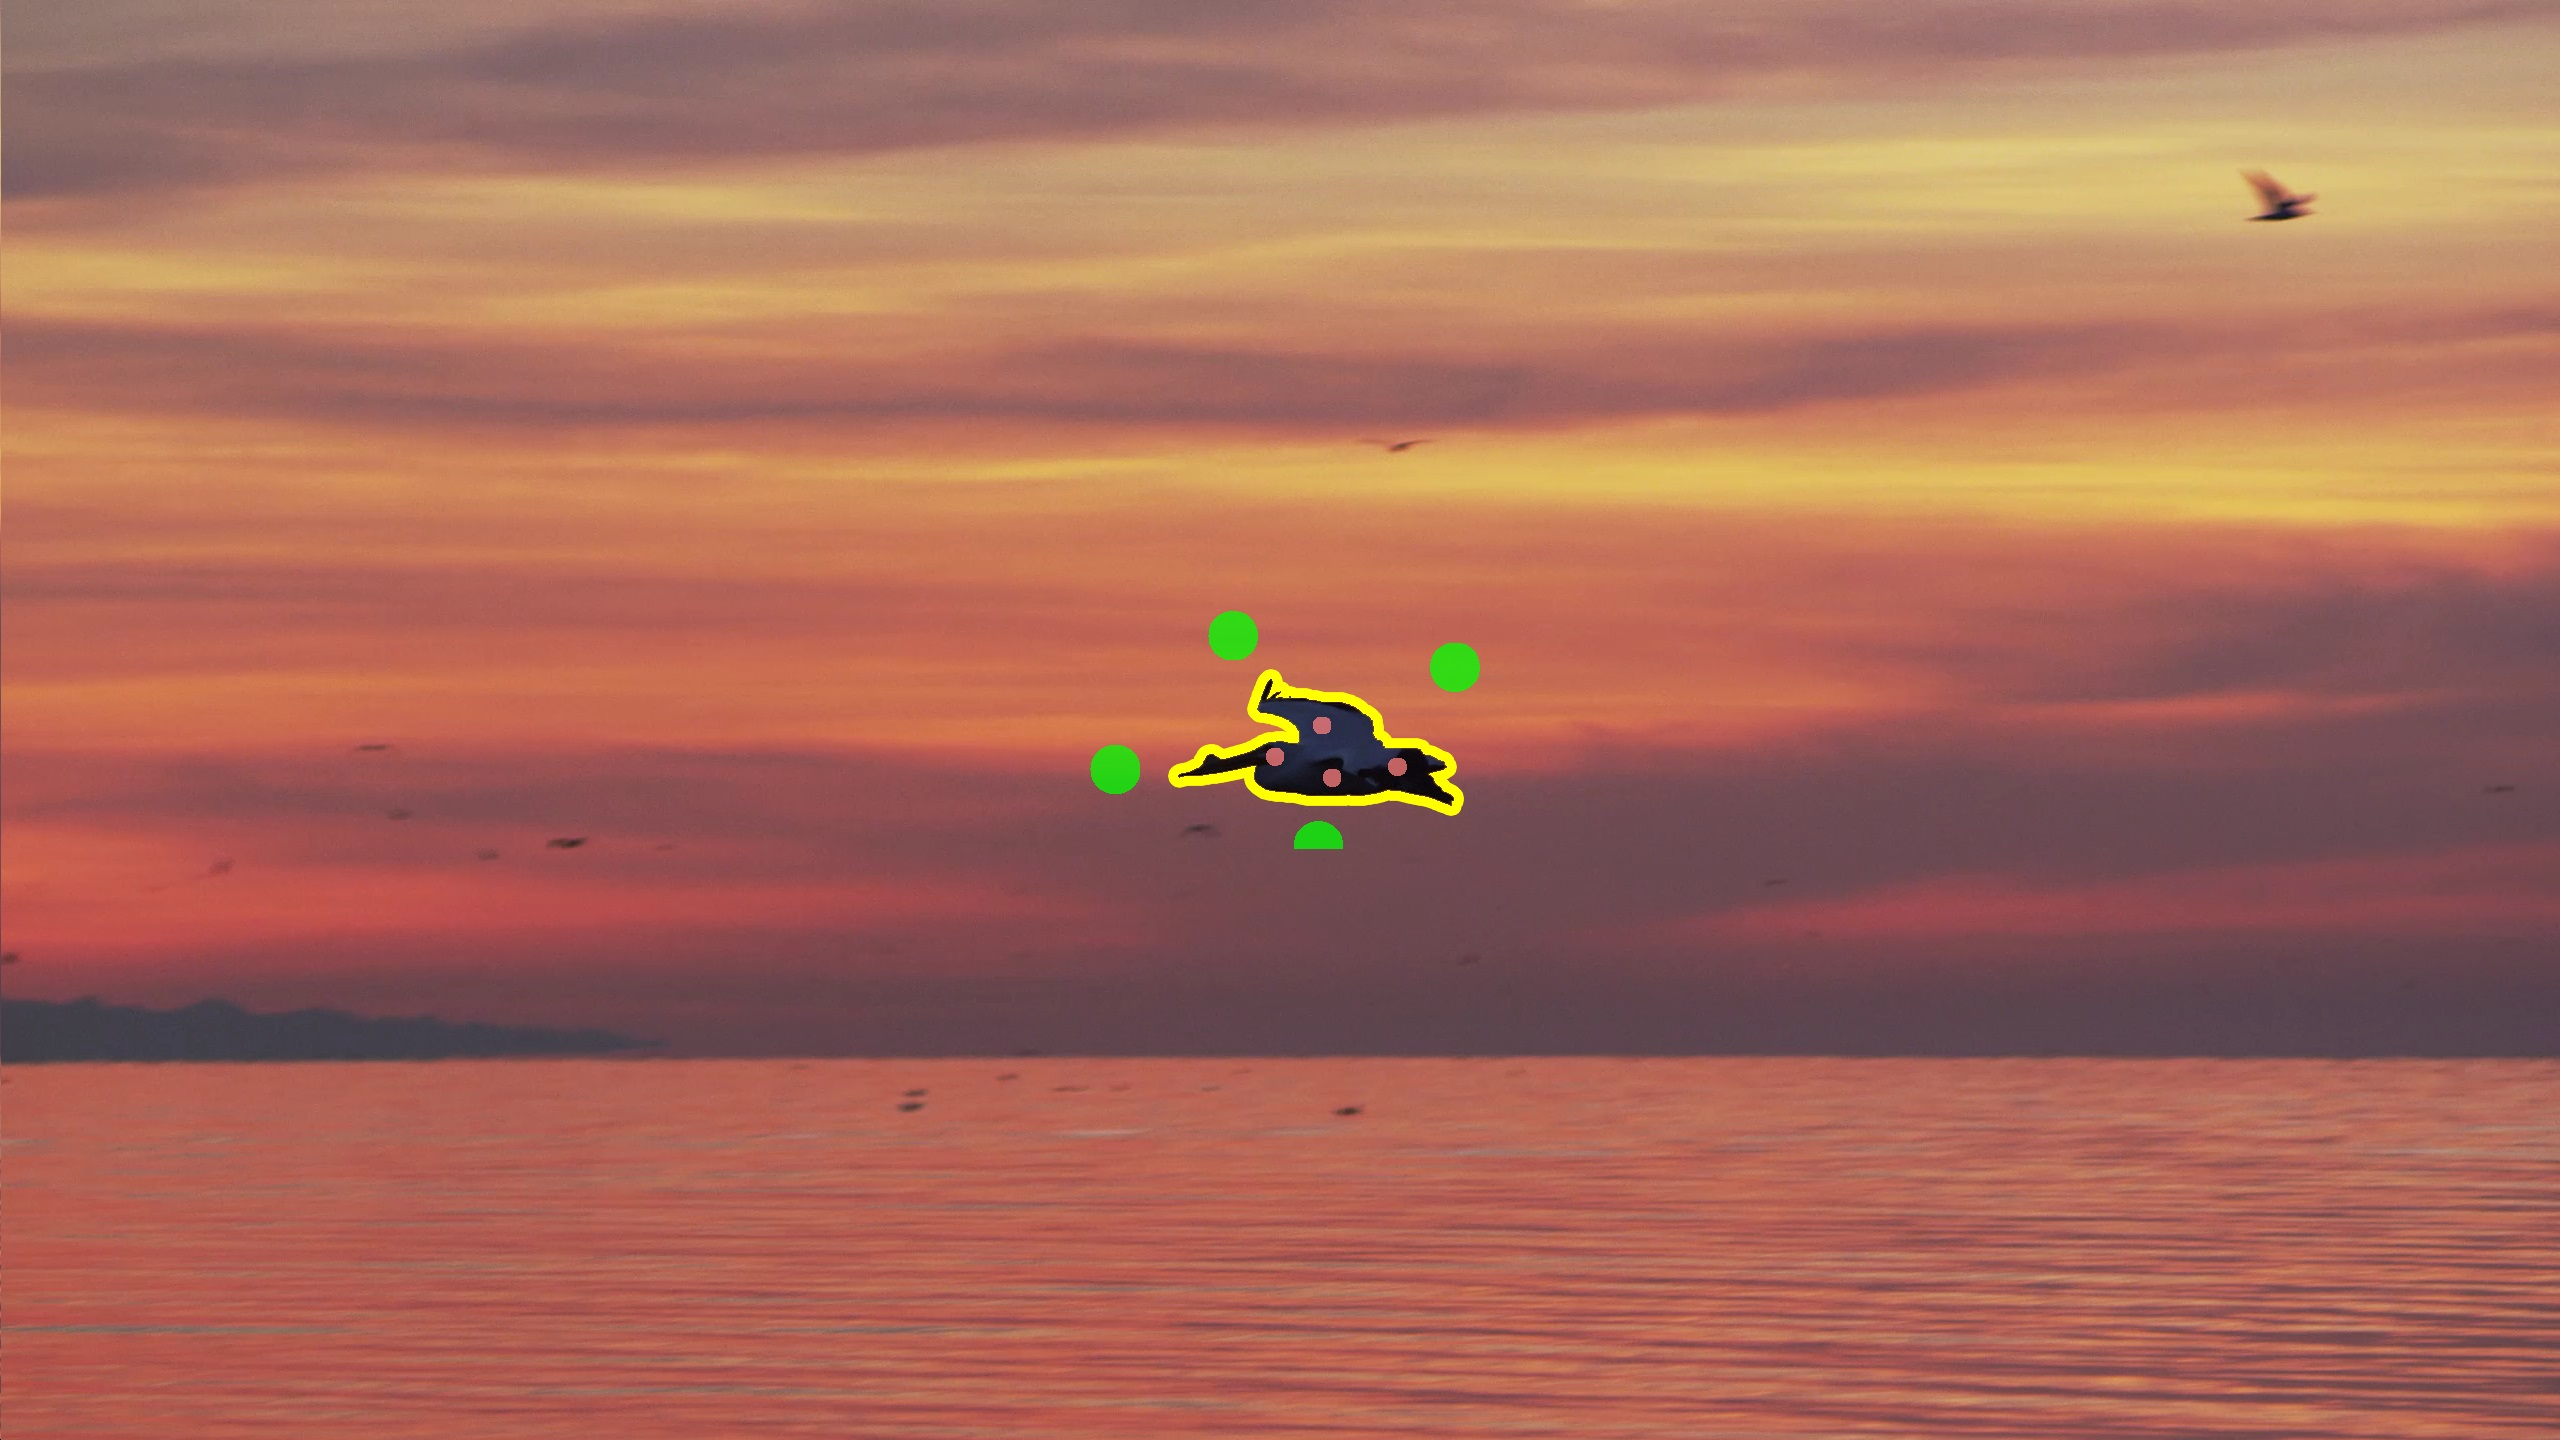
\includegraphics[width=5cm]{figures/fig16b.jpg}
    }
\subfigure[THE CROODS - Frame]{
    \label{figure eep frame}
    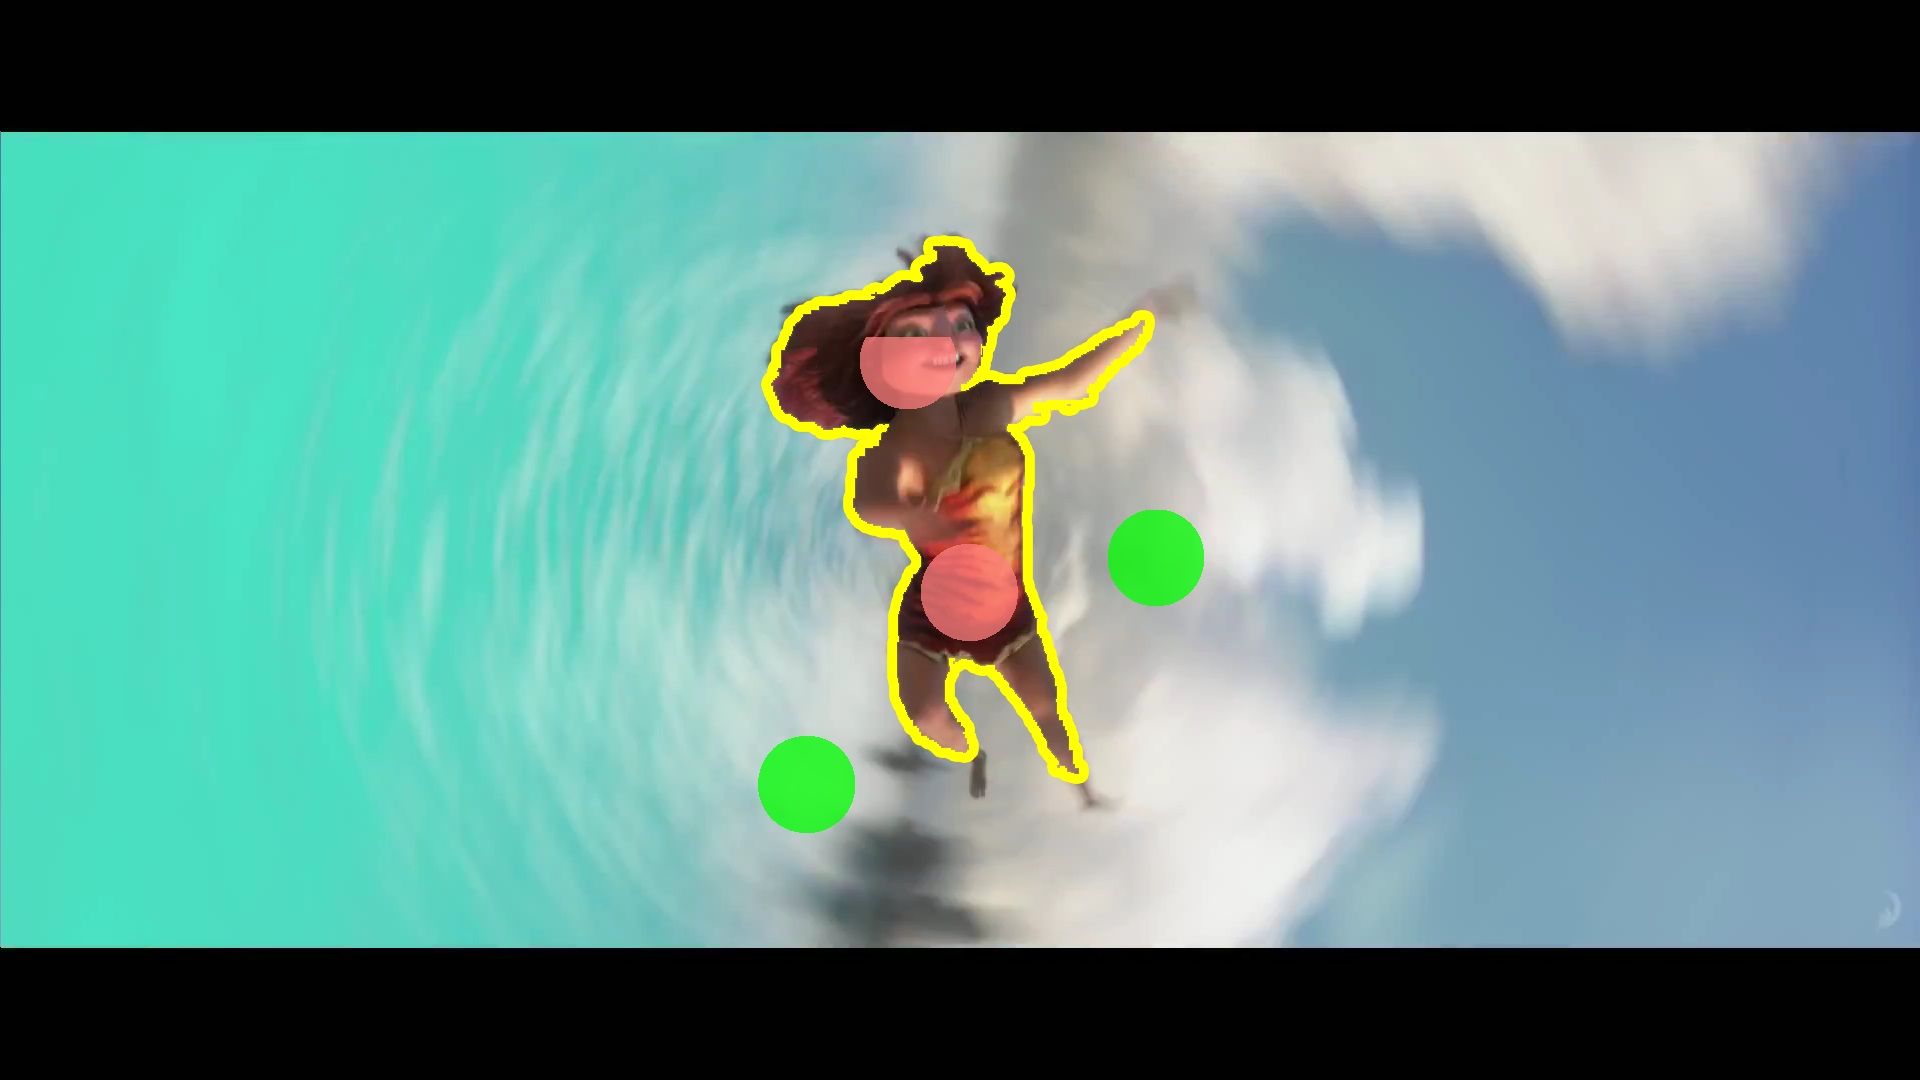
\includegraphics[width=5cm]{figures/fig14b.jpg}
    }
\subfigure[Life of PI - Frame]{
    \label{figure pi frame}
    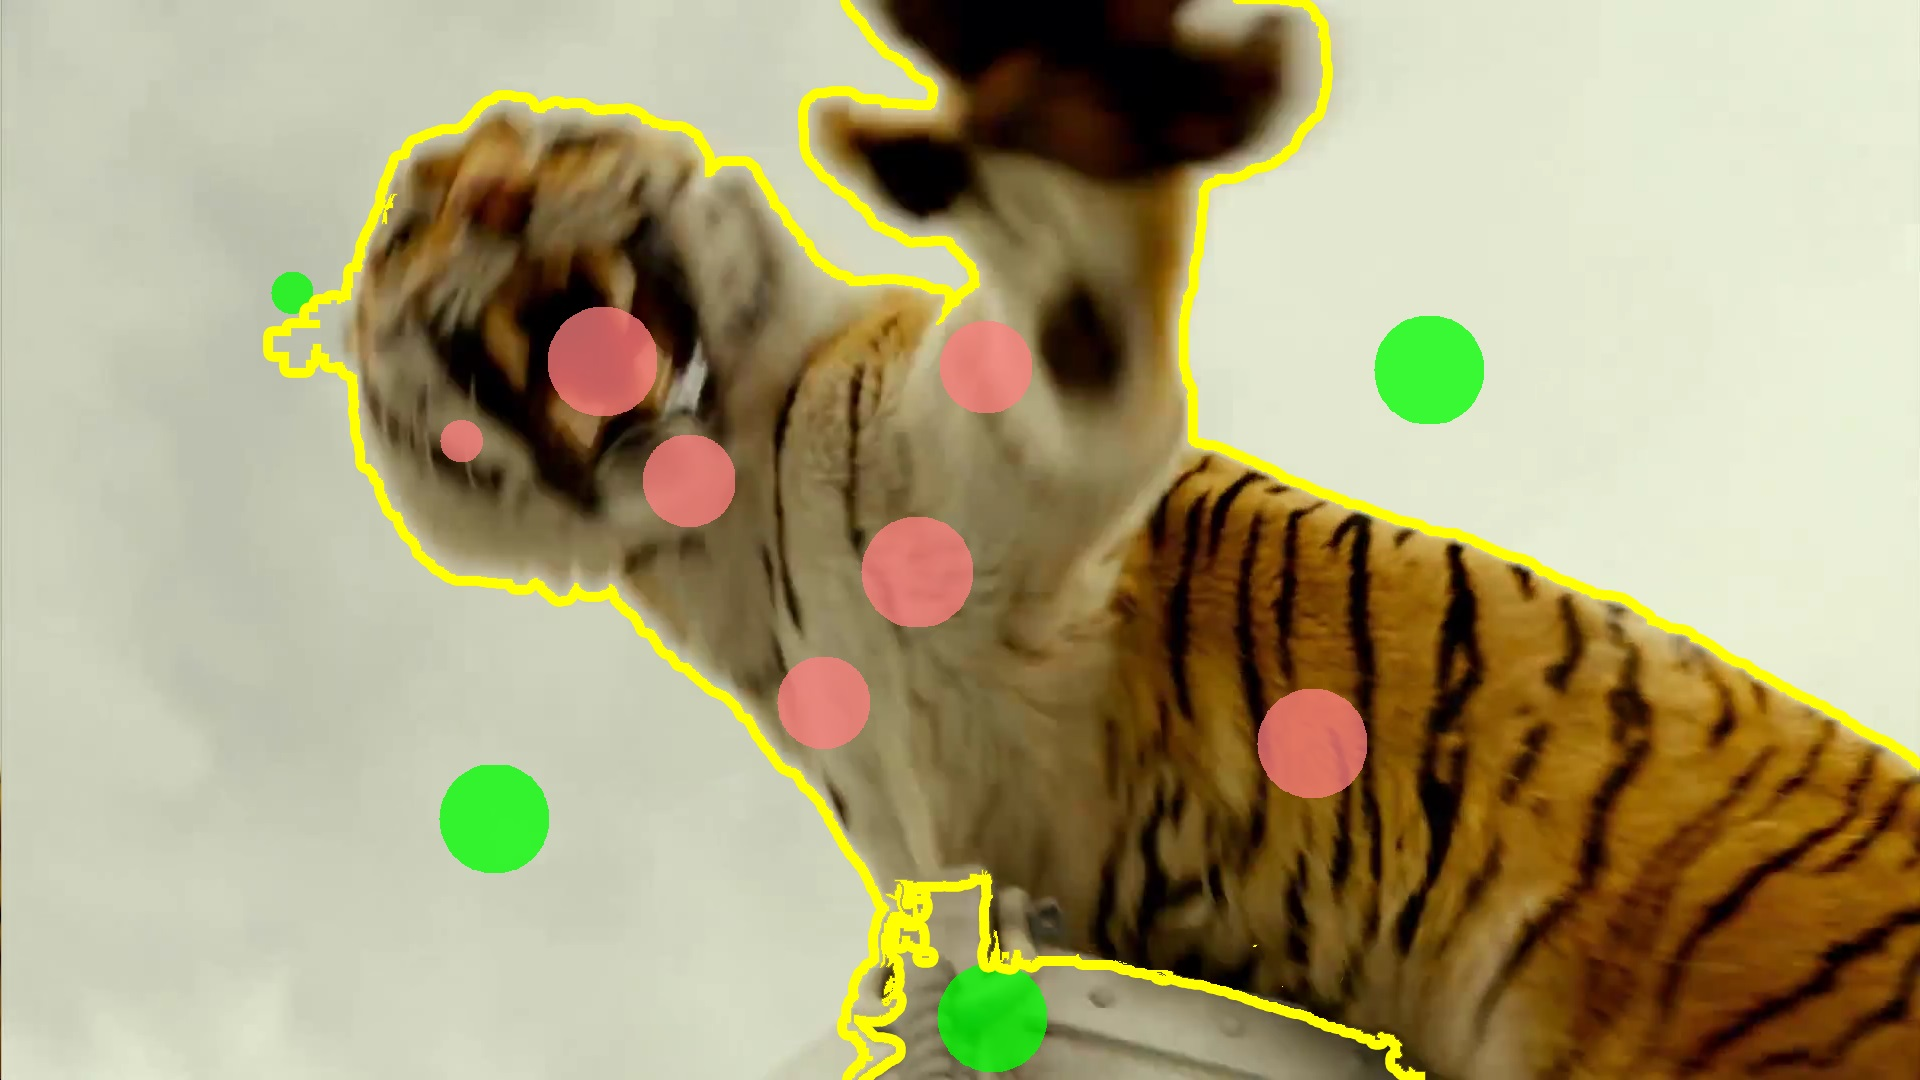
\includegraphics[width=5cm]{figures/fig15b.jpg}
    }
\caption{Video Cutout Results.
\ref{figure 4k 3d}, \ref{figure 4k frame}: the cut-out bird \protect\footnotemark[4].
\ref{figure eep 3d}, \ref{figure eep frame}: the cut-out Eep \protect\footnotemark[5].
\ref{figure pi 3d}, \ref{figure pi frame}: the cut-out tiger \protect\footnotemark[6].
}
\label{figure video cutout}
\end{figure*}

\paragraph*{\textbf{Volume Segmentation}} In terms of scalar field data sets, we use the first model to build an energy function.
Because the augmenting-paths are much longer, the computing costs are much higher compared with images.
The segmentation results of CT
\footnotemark[7]\footnotetext[7]{\scriptsize MRBrain: \url{http://www-graphics.stanford.edu/data/voldata/}} and MRI
\footnotemark[8]\footnotetext[8]{\scriptsize Lobster: \url{http://www.volvis.org/}} data sets are shown in \figurename \ref{figure volume segmentation}.

\begin{figure*}
\centering
\subfigure[MRBrain - $256 \times 256 \times 109$]{
    \label{figure mrbrain}
    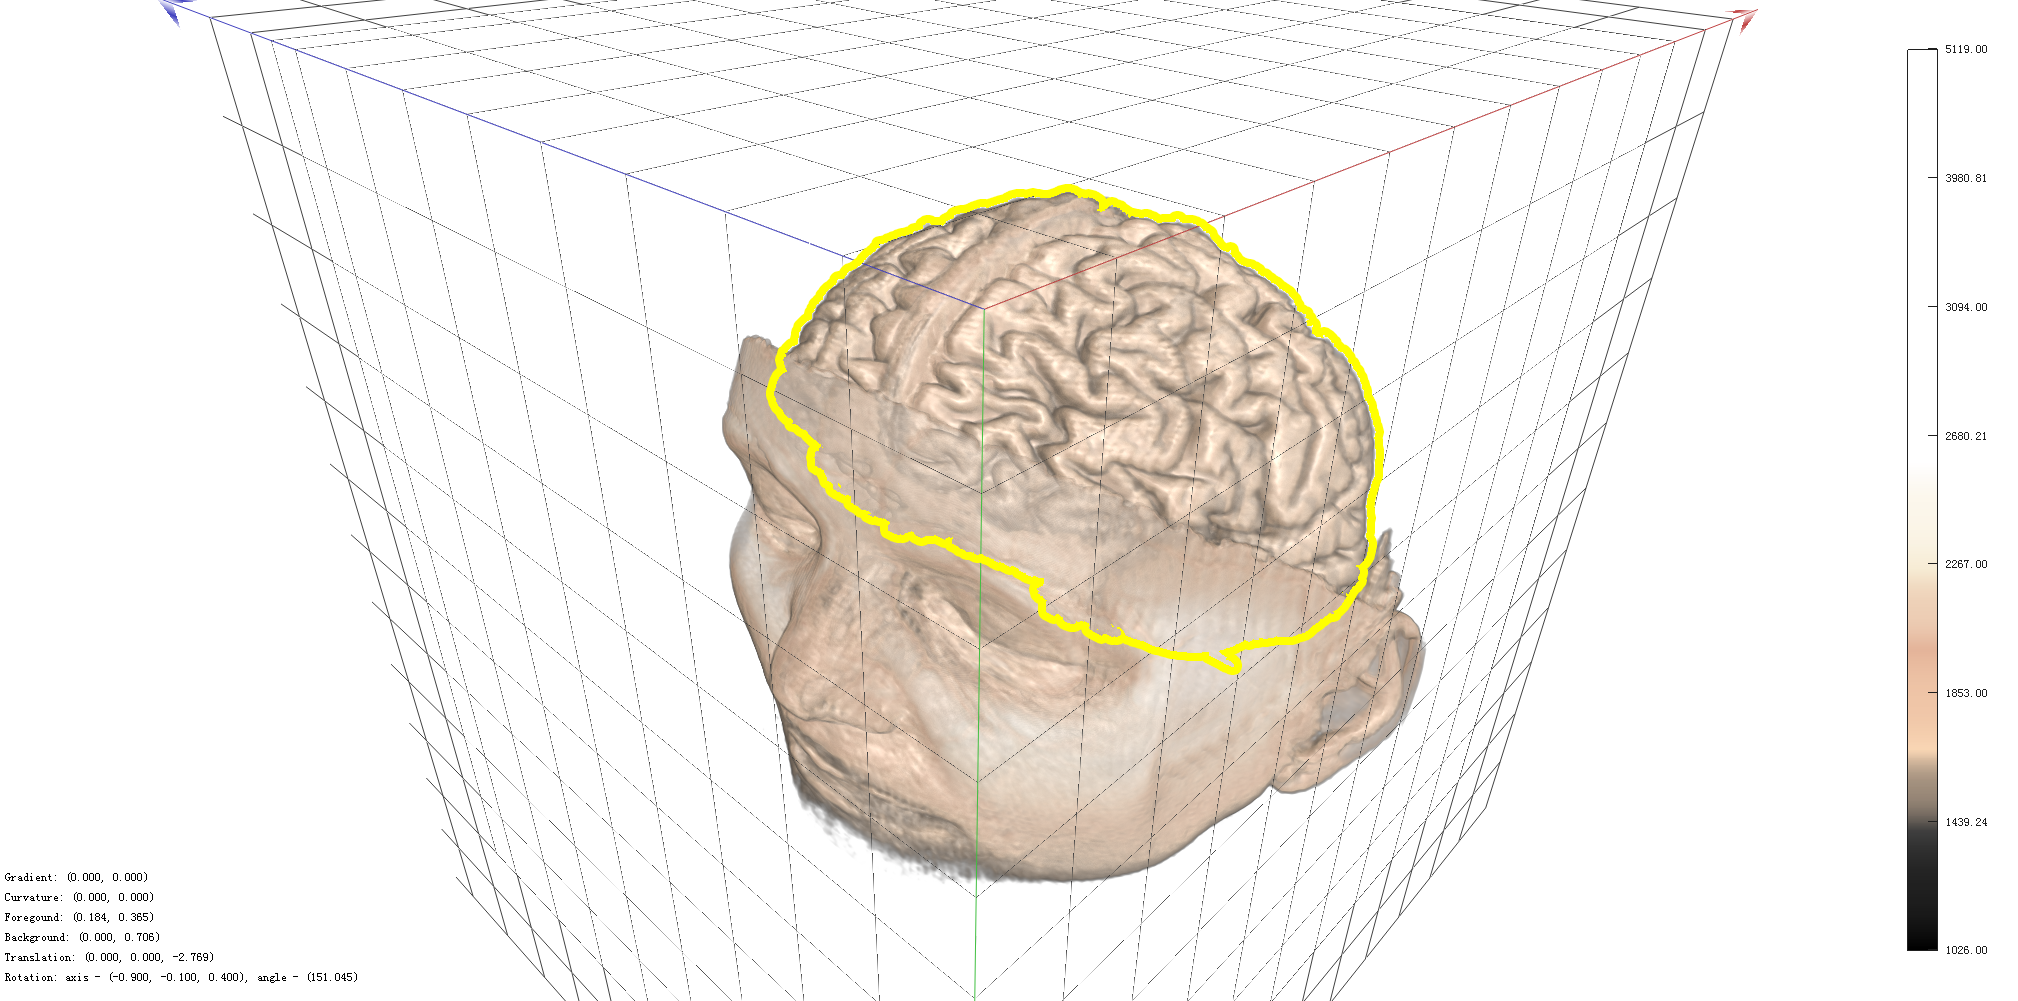
\includegraphics[width=7.5cm]{figures/fig9f.png}
    }
\subfigure[Lobster - $301 \times 324 \times 56$]{
    \label{figure lobster}
    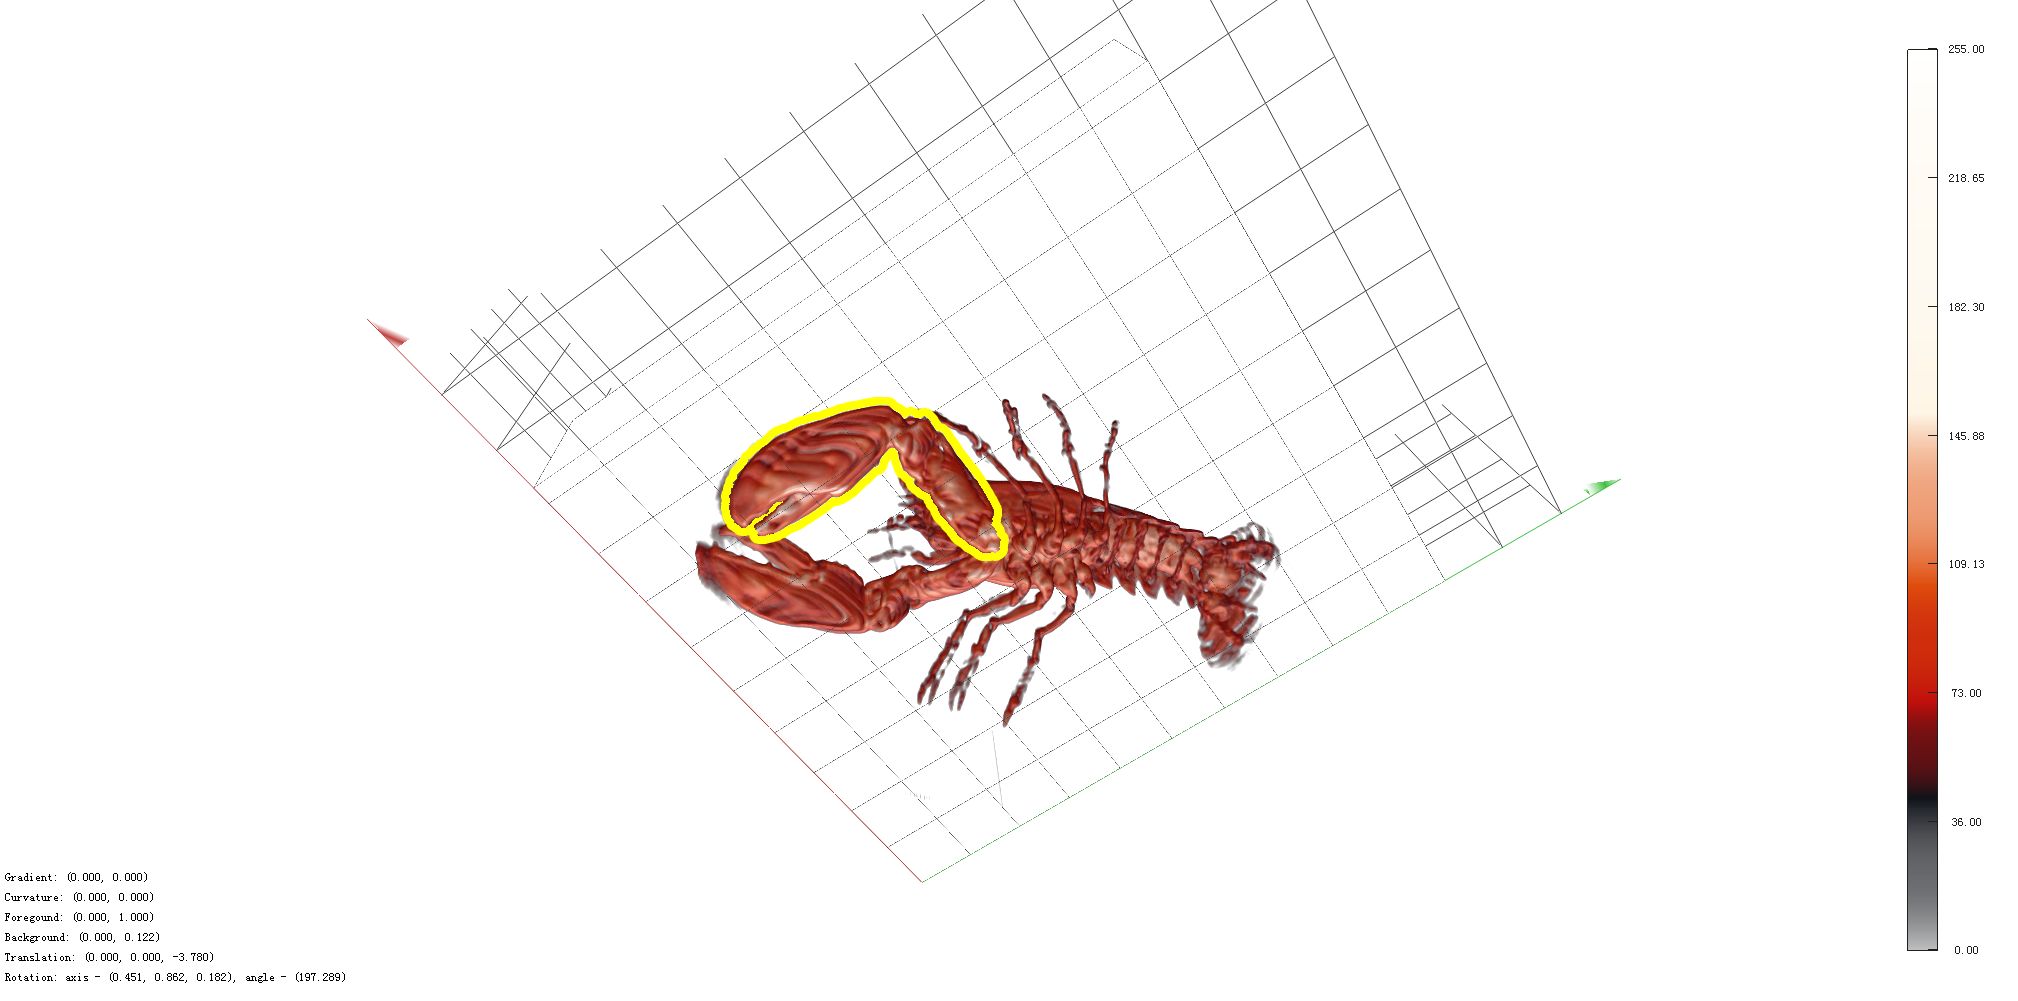
\includegraphics[width=7.5cm]{figures/fig13f.png}
    }
\caption{Volume Segmentation Results.
\ref{figure mrbrain}: MRBrain - MRI and the cutout brain \protect\footnotemark[7].
\ref{figure lobster}: Lobster - CT and the cutout claw \protect\footnotemark[8].
}
\label{figure volume segmentation}
\end{figure*}

%-------------------------------------------------------------------------
\subsection{Performance}

We first compare our method with CUDA-Cut \cite{08VN} and Fast-Cut \cite{09S, 11W} which are GPU based methods, and then with CPU based methods BK \cite{04BK} and Grid-Cut \cite{12JSH}.

\paragraph*{\textbf{GPU Based Methods}}

CUDA-Cut provides two different implementations: atomic (PushPull + Relbel) and stochastic (Push + PullRelabel).
We use the stochastic version for comparison, because it is faster.
We also observe that CUDA-Cut doesn't guarantee global convergence and it often outputs larger energies.
We divide the minimum energy by its output to measure the degree of approximation as listed in the second column of \tablename \ \ref{table gpu performance}.
Because JF-Cut and Fast-Cut always yield global optimal results, their accuracies are not listed.

We implement Fast-Cut using OpenCL and extends it to support videos (some of the optimization techniques are deprecated for generality).
To be fair, we perform global relabel once at the beginning by using the same block size and mainly compare the cost on push-relabel which is the major part of all GPU based methods
(we perform convergence detection and active block counting much less frequently).

\begin{table}
\center
\caption{GPU Based Methods}
\label{table gpu performance}
{
    \fontsize{6.5pt}{7.5pt}\selectfont
    \begin{tabular}{@{ }c|r|r|r|r|r@{ }r@{ }}
    \hline
    Instance & \multicolumn{2}{|c|}{CUDA-Cut} & Fast-Cut & JF-Cut & \multicolumn{2}{c}{Speedup} \\
    \hline
    Name        & Accuracy & Time(ms) & Time(ms) & Time(ms) & -/CUDA & -/Fast\\
    \hline
    flower      & 0.736 & 48.6  & 9.7       & 4.2       & 11.5  & 2.3\\
    4 x 4       & 0.673 & 622.2 & 262.4     & 90.0      & 6.9   & 2.9\\
    16 x 16     & -     & -     & 9636.7    & 2192.3    & -     & 4.4\\
    person      & 0.358 & 73.9  & 20.9      & 10.0      & 7.4   & 2.1\\
    4 x 4       & 0.674 & 612.0 & 290.9     & 120.7     & 5.1   & 2.4\\
    16 x 16     & -     & -     & 12131.0   & 3403.6    & -     & 3.6\\
    sponge      & 1.000 & 48.7  & 5.4       & 4.4       & 11.0  & 1.2\\
    4 x 4       & 0.973 & 637.3 & 151.7     & 31.4      & 20.3  & 4.8\\
    16 x 16     & -     & -     & 3689.5    & 595.3     & -     & 6.2\\
    \hline
    bone        & -     & -     & 5643.6    & 616.9     & -     & 9.1\\
    2 x 2 x 2   & -     & -     & 68712.3   & 6749.9    & -     & 10.2\\
    liver       & -     & -     & 6211.4    & 585.7     & -     & 10.6\\
    2 x 2 x 2   & -     & -     & 165704.3  & 16441.2   & -     & 10.1\\
    babyface    & -     & -     & 7932.5    & 830.2     & -     & 9.6\\
    2 x 2 x 2   & -     & -     & 104277.6  & 11309.2   & -     & 9.2\\
    adhead      & -     & -     & 17084.4   & 1654.6    & -     & 10.3\\
    2 x 2 x 2   & -     & -     & 115991.0  & 10511.7   & -     & 11.0\\
    \hline
    madagascar  & -     & -     & 49559.9   & 24465.4   & -     & 2.0\\
    lta         & -     & -     & 95605.9   & 51279.0   & -     & 1.9\\
    \hline
    timescapes  & -     & -     & 357.2     & 78.6      & -     & 4.5\\
    the croods  & -     & -     & 9410.7    & 1374.6    & -     & 6.8\\
    life of pi  & -     & -     & 743.4     & 80.9      & -     & 9.2\\
    \hline
    mrbrain     & -     & -     & 9381.0    & 1226.2    & -     & 7.7\\
    lobster     & -     & -     & 2892.9    & 321.5     & -     & 9.0\\
    \hline
    \end{tabular}
    \begin{tablenotes}
        \item {
        \begin{enumerate}
            \item CUDA-Cut (v1.0) - \url{http://cvit.iiit.ac.in/resources/cudacuts/}
            \item Environment - Nvidia GeForce GTX TITAN
        \end{enumerate}}
    \end{tablenotes}
}
\end{table}

\tablename \ \ref{table gpu performance} shows the performance of CUDA-Cut, Fast-Cut and our method with millisecond precision.
Because CUDA-Cut consumes too much memory, it cannot handle large date sets, even there are 6GB device memory.
For all data sets listed in \tablename \ \ref{table benchmark}, JF-Cut is faster than Fast-Cut and CUDA-Cut.
Our method achieves a maximum 20-fold speedup, see Sponge $4 \times 4$.
Larger data sets lead to higher speedups, which means our approach is more suitable for large data sets.

\begin{table}
\center
\caption{Convergence Speed}
\label{table convergence speed}
{
    \fontsize{6.5pt}{7.5pt}\selectfont
    \begin{tabular}{@{ }c|r@{ }r@{ }r|r@{ }r@{ }}
    \hline
    Instance & \multicolumn{3}{|c|}{Iterations} & \multicolumn{2}{c}{Ratios}\\
    \hline
    Name & CUDA & Fast-Cut & JF-Cut & -/CUDA & -/Fast\\
    \hline
    flower      & 155   & 41    & 10    & 15.5  & 4.1\\
    4 x 4       & 232   & 174   & 81    & 2.9   & 2.1\\
    16 x 16     & -     & 516   & 195   & -     & 2.6\\
    person      & 232   & 100   & 26    & 8.9   & 3.8\\
    4 x 4       & 232   & 203   & 88    & 2.6   & 2.3\\
    16 x 16     & -     & 692   & 366   & -     & 1.9\\
    sponge      & 155   & 31    & 14    & 11.1  & 2.2\\
    4 x 4       & 232   & 114   & 27    & 8.6   & 4.2\\
    16 x 16     & -     & 234   & 84    & -     & 2.8\\
    \hline
    bone        & -     & 265   & 125   & -     & 2.1\\
    2 x 2 x 2   & -     & 410   & 184   & -     & 2.2\\
    liver       & -     & 498   & 170   & -     & 2.9\\
    2 x 2 x 2   & -     & 1721  & 697   & -     & 2.5\\
    babyface    & -     & 512   & 194   & -     & 2.6\\
    2 x 2 x 2   & -     & 876   & 413   & -     & 2.1\\
    adhead      & -     & 518   & 197   & -     & 2.6\\
    2 x 2 x 2   & -     & 439   & 175   & -     & 2.5\\
    \hline
    madagascar  & -     & 1344  & 609   & -     & 2.2\\
    lta         & -     & 1344  & 668   & -     & 2.0\\
    \hline
    timescapes  & -     & 36    & 13    & -     & 2.8\\
    the croods  & -     & 68    & 34    & -     & 2.0\\
    life of pi  & -     & 32    & 10    & -     & 3.2\\
    \hline
    mrbrain     & -     & 516   & 282   & -     & 1.8\\
    lobster     & -     & 214   & 104   & -     & 2.1\\
    \hline
    \end{tabular}
}
\end{table}

The convergence speed of different methods is shown in \tablename \ \ref{table convergence speed}.
Because the augmenting paths in volume data sets are longer than in images, volume data sets need more iterations.
Our method has higher convergence speeds which are more than twice the rates of Fast-Cut and almost 10-fold to CUDA-Cut.

\paragraph*{\textbf{CPU Based Methods}}

We download the latest version of BK (V3.03) and Grid-Cut (V1.1) and compile them to get the 64-bit programs.
The reason why we choose 64-bit programs is that for large data sets, such as adhead $2 \times 2 \times 2$ and TimeScapes, BK requires a contiguous memory which is larger than 4GB.
We use the same compiler settings for comparison, see the table notes in \tablename \ \ref{table cpu performance}.

\begin{table}
\caption{CPU Based Methods}
\label{table cpu performance}
{
    \fontsize{6.5pt}{7.5pt}\selectfont
    \begin{tabular}{@{ }c|r|r@{ }r|r@{ }r@{ }r@{ }r@{ }}
    \hline
    Instance & BK & \multicolumn{2}{c}{Grid-Cut} & \multicolumn{4}{c}{JF-Cut}\\
    \hline
    Name        & Total     & 1 Thread & 8 Threads & Total & -/BK  & -/GC-1 & -/GC-8\\
    \hline
    flower      & 29        & 18     & 6       & 6     & 4.7   & 2.9    & 1.0\\
    4 x 4       & 495       & 131    & 89      & 101   & 4.9   & 1.3    & 0.9\\
    16 x 16     & 9850      & 2392   & 1462    & 1575  & 6.3   & 1.5    & 0.9\\
    person      & 29        & 9      & 7       & 14    & 2.1   & 0.6    & 0.5\\
    4 x 4       & 494       & 121    & 92      & 118   & 4.2   & 1.0    & 0.8\\
    16 x 16     & 9111      & 2069   & 1377    & 2417  & 3.8   & 0.9    & 0.6\\
    sponge      & 28        & 7      & 6       & 13    & 2.2   & 0.6    & 0.5\\
    4 x 4       & 466       & 93     & 79      & 41    & 11.5  & 2.3    & 1.9\\
    16 x 16     & 7537      & 1531   & 1265    & 595   & 12.7  & 2.6    & 2.1\\
    \hline
    bone        & 5761      & 867    & 519     & 421   & 13.7  & 2.1    & 1.2\\
    2 x 2 x 2   & 204874    & 32057  & 20402   & 4707  & 43.5  & 6.8    & 4.3\\
    liver       & 10769     & 3254   & 3916    & 305   & 35.3  & 10.7   & 12.8\\
    2 x 2 x 2   & 855279    & 237593 & 256249  & 7923  & 107.9 & 30.0   & 32.3\\
    babyface    & 8940      & 2619   & 1501    & 459   & 19.5  & 5.7    & 3.3\\
    2 x 2 x 2   & 809026    & 231592 & 233656  & 5825  & 138.9 & 39.8   & 40.1\\
    adhead      & 23192     & 6517   & 4149    & 980   & 23.7  & 6.6    & 4.2\\
    2 x 2 x 2   & 223934    & 41414  & 21274   & 7921  & 28.3  & 5.2    & 2.7\\
    \hline
    madagascar  & 114673    & 29658  & 12269   & 13730 & 8.4   & 2.2    & 0.9\\
    lta         & 104006    & 32055  & 13139   & 24275 & 4.3   & 1.3    & 0.5\\
    \hline
    timescapes  & 18175     & 3640   & 2741    & -     & -     & -      & -\\
    the croods  & 12603     & 2883   & 2115    & 906   & 13.9  & 3.2    & 2.3\\
    life of pi  & 11700     & 3925   & 2162    & 209   & 55.9  & 18.8   & 10.3\\
    \hline
    mrbrain     & 3902      & 599    & 597     & 798   & 4.9   & 0.8    & 0.7\\
    lobster     & 7028      & 1428   & 657     & 229   & 30.7  & 6.2    & 2.9\\
    \hline
    \end{tabular}
    \begin{tablenotes}
        \item {
        \begin{enumerate}
            \item BK (v3.03) - \url{http://pub.ist.ac.at/~vnk/software.html}
            \item Grid-Cut (v1.1) - \url{http://gridcut.com/downloads.php}
            \item Compiler Settings for GCC (v4.9.0) -O3 -march=native -mtune=generic -DNDEBUG
            \item Environment - Intel (R) Core i7-3770 and AMD Radeon HD 7990
        \end{enumerate}}
    \end{tablenotes}
}
\end{table}

\tablename \ \ref{table cpu performance} compares the performance of BK, Grid-Cut and our method.
Our method's speedup over Gird-Cut increases with the data scale, except for some data sets.
Compared with Grid-Cut, we achieve a maximum 3-fold speedup (sponge $16 \times 16$) for images, a 20-fold speed up (life of pi) for videos and a 40-fold speedup (babyface $2 \times 2 \times 2$) for volume data sets.
With its parallel version (8 threads), the maximum speedups are 2-fold for images, 10-fold for videos and 40-fold for volume data sets.

We also observe that there exists a notable variant.
The decisive factor may be the graph topology.
The reason is that in volume data sets most of the terminal-edges have zero capacities, while in images most of them are positive, which will greatly affect the convergence speed.
These speedups are lower than of GPU based methods, because there exist big differences between CPU based methods (based on augmenting-path) and GPU based methods (based on push-relabel).
In summary, for large data sets our method significantly outperforms other methods.



%-------------------------------------------------------------------------
\section{Discussions}
\label{section discussions}

We analyze our tuning techniques and discuss the quality and the limitations of our approach.

\subsection{\textbf{Convergence Proof}}

The standard push-relabel method \cite{88GT} maintains a preflow and always keeps a valid labeling:

\begin{itemize}
\item[-] \textbf{Definition 1 (Preflow)} An assignment of a non-negative flow $f(u, v)$ to each edge $(u, v)$ of a network $(G = (V, E), s, t, c)$ is a preflow if for each edge $(u, v)$, $f(u, v) \le c(u, v)$ and for each vertex $v \in V - {t}$, $\sum_{u}f(u, v) - \sum_{w}f(v, w) \ge 0$.
\item[-] \textbf{Definition 2 (Excess Flow)} The excess flow at $v$ is defined as $e_f(v) = \sum_{u}f(u, v) - \sum_{w}f(v, w)$.
\item[-] \textbf{Definition 3 (Invariant)} At every step, if there is an edge $(u, v)$ that has a positive capacity $c'(u, v) > 0$ in the residual network, then $h(u) \le h(v) + 1$ and this labeling is $valid$.
\end{itemize}

The standard method consists of two steps: initialization and the main loop.
In the first step, it saturates all the edges $(s, v) \in E$ from the source $s$ and sets the original labeling $h(s) = n$, $h(v) = 0$ for all $v \in V$, $v \ne s$.
This gives a valid preflow $f_0$.
In the main loop, for each active node $u$, perform the following push and relabel operations:

\begin{itemize}
\item[-] \textbf{Push}(u) \  If $\exists v$ with admissible arc $(u, v) \in E_f$, then send flow $\delta \gets \min(c_f(u, v), e_f(u))$ from $u$ to $v$.
\item[-] \textbf{Relabel}(u) \  If for all arcs $(u, v)$ out of $u$, either $(u, v) \notin E_f$ or $h(v) \ge h(u)$, then set $h(u) = 1 + \min_{v:(u,v) \in E_f} h(v)$.
\end{itemize}

In our method, we take the initialization step and do push or relabel in a specific order until there is no augmenting $s-t$ path (ensured by the convergence detection).
Three lemmas are provided below to prove the convergence of our algorithm:

\begin{itemize}
\item[-] \textbf{Lemma 1} The labels $h$ remain valid in \textbf{H4} (the last step of our method in Section \ref{section hpr}).
\item[] \textbf{Proof:}
The proof is done by induction.
Initially $h$ is valid with respect to $f_0$.
In \textbf{H4}, we perform push and relabel operations alternatively.
When we push a node on the admissible arc $(u, v)$, the new arc $(v, u) \in E_f$ satisfies $d(v) = d(u) - 1 \le d(u) + 1$ and the labels remain valid.
When we relabel a node, the new label is the largest one while remaining valid.
Because each operation is independent (no data conflict), the property remains true.

\item[-] \textbf{Lemma 2} The push-relabel given by \textbf{H3} is equivalent to the original push-relabel algorithm.
\item[] \textbf{Proof:}
In our method, each operation (push or relabel) is the same as the standard one and we perform these operations in parallel.
In \textbf{H3}, we process even blocks and odd blocks alternatively.
For each block, we relabel even nodes and odd nodes respectively, and then push them in the same way.
This ensures that, there is no data conflict and all the operations are independent.
And there exists at least one sequential way to perform these operations to get the same results.
Note that in the original method, changing the processing order does not affect the convergence.
Thus, our method is equivalent to the original push-relabel algorithm.

\item[-] \textbf{Lemma 3} The final preflow resulted from \textbf{H2} is a maximum flow.
\item[] \textbf{Proof:}
In \textbf{H2}, we start from the foreground nodes and repeat expanding them in the residual graph.
If the algorithm terminates without finding any background node, then there is no augmenting-path.
Hence the final preflow is a maximum flow.
\end{itemize}

Overall, these lemmas prove that our method can yield global optimal results like the standard push-relabel algorithm.

\subsection{\textbf{Complexity Analysis}}

The complexity of the original push-relabel algorithm is $O(V^2 E)$.
Most GPU based methods are based on it and use different strategies to process active nodes to improve the performance.
However, the accurate analysis is quite difficult.
As the access of global memory ($400-600$ cycles) is much slower than shared memory ($20-40$ cycles), we can use the workload per global memory read/write as metric to compare different methods.

\begin{itemize}
\item[-] \textbf{Metric 1} The first metric $N$ is the number of operations (push or relabel) per global memory read/write. A larger $N$ means a lower complexity.
\item[-] \textbf{Metric 2} The second metric $D$ is the propagation distance of a flow per global memory read/write. A larger $D$ means a lower complexity.
\end{itemize}

\begin{table}
\center
\caption{Complexity Analysis}
\label{table complexity analysis}
{
    \fontsize{6.5pt}{7.5pt}\selectfont
    \begin{tabular}{@{ }c|c|c|c|c|c@{ }}
    \hline
    Metric   & Dimension & Block Size & \multicolumn{2}{c}{Wave Push} & \multicolumn{1}{c}{Block-Wise}\\
    \hline
    -   & - & -         & CUDA & Fast-Cut & JF-Cut\\
    \hline
    $N$ & 2 & -         & 0.25 & 0.25 & 4    \\
    $N$ & 3 & -         & -    & 0.13 & 6    \\
    \hline
    $D$ & 2 & 16 x 16   & 16   & 16   & 256  \\
    $D$ & 2 & 32 x 32   & 32   & 32   & 1024 \\
    $D$ & 3 & 4 x 4 x 4 & -    & 4    & 64   \\
    $D$ & 3 & 8 x 8 x 8 & -    & 8    & 512  \\
    \hline
    \end{tabular}
}
\end{table}

In terms of \textbf{Metric 1}, because CUDA-Cut and Fast-Cut perform a Wave Push, they can perform at most $N=\frac{1}{2d}$ operations (push or relabel in all the directoins) within one global memory read/write, where $d$ denotes the dimension.
The reason is that, for each direction, one operation (push or relabel) in their method needs at least one global memory read/write.
In our method, for one node, we can perform at least $N'=2d$ operations within one global memory read/write (see \tablename \ \ref{table complexity analysis}).

In terms of \textbf{Metric 2}, for one block, CUDA-Cut and Fast-Cut can send a flow along $D=\max{\{x, y, z\}}$ edges at most in one direction within one global memory read/write, where $(x, y, z)$ denotes the block size.
However, we can send a flow from one node to any other node in the same block, which means in one global memory read/write, the maximum propagation distance of a flow that we can achieve is $D'=x \times y \times z$.

\tablename \ \ref{table gpu performance} shows that the workload per global memory read/write in our method is much larger than the ones in others.
Although the worst-case complexity of our algorithm is $O(V^2 E)$ which is the same as CUDA-Cut and Fast-Cut.
The average running time of our method is $n = \frac{N'D'}{ND} \approx \frac{4d^2xyz}{\max{\{x, y, z\}}}$ times faster than CUDA-Cut and Fast-Cut.
We increase the information propagation speed throughout the block.
Ours leads to a fast convergence and a lower complexity compared with CUDA-Cut and Fast-Cut (see \tablename \ \ref{table convergence speed}).

\subsection{\textbf{Quality}}

Compared with CUDA-Cut, our approach guarantees the global minimal, meaning that we can get the optimal results.
For images such as Flower and Person (see \tablename \ \ref{table gpu performance}), CUDA-Cut yields inaccurate results.
This means that the underlying flow is less than the maximum one (see the Person data set, for which the accuracy is only 0.358).
This is because CUDA-Cut does not check the convergence and stops iterating after a specific number of iterations before reaching the global optimum.
In contrast, JF-Cut, Fast-Cut, BK and Grid-Cut guarantee the global optimum and the maximum flow they get are the same, as shown in \tablename \ \ref{table benchmark}.

In practice, given the same model (the way of defining excess flow and edge capacity), these methods get the same segmentation boundaries due to the global convergence (see \figurename \ref{figure image segmentation} and \figurename \ref{figure video cutout}).
Moreover, we use in-block push-relabel to improve the speed of information propagation, achieve a fast convergence compared with Fast-Cut.
In this sense our approach can handle large data sets more efficiently and yields more practical results (https://github.com/15pengyi/JF-Cut).

\subsection{\textbf{Algorithm Tuning}}

For better performance, we develop a 2D version of our approach to handle images.
And the parameter settings are different for small data sets and large data sets.
When the data sets are small, we use $(k_1, k_2) = (4, 2)$ to increase the frequency of active block counting to ensure fewer iterations.
For large data sets, $(k_1, k_2)$ is set to $(16, 4)$ to reduce the cost of both active block counting and convergence detection.

Other optimizations include using local memory to cache the data which have multiple read or write per execution, checking if the value has changed before writing, using \textit{SOA} (Structure of Array) instead of \textit{AOS} (Array of Structures) and designing a compact structure (four bytes per unit) to support a coalesced read and write for global memory and avoid bank conflicts.
We also use \textit{AMD APP Profiler} and \textit{NVIDIA Visual Profiler} to help us identify performance bottlenecks.

\subsection{\textbf{Limitations}}

Our approach has several limitations compared with CPU-based methods.
First, the feasible data size of our approach is limited by GPU memory, i.e., \textit{CL\_DEVICE\_GLOBAL\_MEM\_SIZE} and \textit{CL\_DEVICE\_MAX\_MEM\_ALLOC\_SIZE} which are defined by the OpenCL environment.
For \textit{GeForce GTX TITAN} and \textit{AMD Radeon HD 7990} these parameters are (6GB, 1.5GB) and (3GB, 512MB) respectively.
Instead, the size of contiguous-memory on the CPU can be much larger, e.g. 32GB.
In addition, GPU based methods have to copy data from host memory to device memory, which consumes extra time.
Compared with BK techniques that are affordable for unstructured data, our method currently only supports structured data.

To overcome the limitation of GPU memory, extremely large data can be partitioned and distributed on the GPU clusters.
In terms of unstructured data, we need to convert the unstructured grid into a hierarchy of regular grids and perform JF-Cut in different levels.


%-------------------------------------------------------------------------
\section{CONCLUSION}
\label{section conclusion}

In this paper, we introduce a parallel graph cut approach named JF-Cut to handle large data sets which has two main advantages:

\begin{enumerate}
\item improving the performance of graph cut for large images and videos using a GPU-based graph cut scheme based on jump flooding, heuristic push /relabel and convergence detection;
\item providing users an interactive graph cut based data segmentation interface that allows for intuitive data selection, interaction and segmentation for large data sets.
\end{enumerate}

We use a variety of data sets (both a benchmark and different large data sets) to evaluate the performance of our approach.
The results show that our method achieves a maximum 40-fold (139-fold) speedup over conventional GPU- (CPU-) based approaches and can be effectively used in different scenarios.
The source code of JF-Cut will be soon available at https://github.com/15pengyi/JF-Cut.

Our future work includes extending our approach to support unstructured data, optimizing the codes and making an independent library for end users to use.


% Computer Society journal papers do something a tad strange with the very
% first section heading (almost always called "Introduction"). They place it
% ABOVE the main text! IEEEtran.cls currently does not do this for you.
% However, You can achieve this effect by making LaTeX jump through some
% hoops via something like:
%
%\ifCLASSOPTIONcompsoc
%  \noindent\raisebox{2\baselineskip}[0pt][0pt]%
%  {\parbox{\columnwidth}{\section{Introduction}\label{sec:introduction}%
%  \global\everypar=\everypar}}%
%  \vspace{-1\baselineskip}\vspace{-\parskip}\par
%\else
%  \section{Introduction}\label{sec:introduction}\par
%\fi
%
% Admittedly, this is a hack and may well be fragile, but seems to do the
% trick for me. Note the need to keep any \label that may be used right
% after \section in the above as the hack puts \section within a raised box.



% The very first letter is a 2 line initial drop letter followed
% by the rest of the first word in caps (small caps for compsoc).
%
% form to use if the first word consists of a single letter:
% \IEEEPARstart{A}{demo} file is ....
%
% form to use if you need the single drop letter followed by
% normal text (unknown if ever used by IEEE):
% \IEEEPARstart{A}{}demo file is ....
%
% Some journals put the first two words in caps:
% \IEEEPARstart{T}{his demo} file is ....
%
% Here we have the typical use of a "T" for an initial drop letter
% and "HIS" in caps to complete the first word.

% You must have at least 2 lines in the paragraph with the drop letter
% (should never be an issue)

% needed in second column of first page if using \IEEEpubid
%\IEEEpubidadjcol

% An example of a floating figure using the graphicx package.
% Note that \label must occur AFTER (or within) \caption.
% For figures, \caption should occur after the \includegraphics.
% Note that IEEEtran v1.7 and later has special internal code that
% is designed to preserve the operation of \label within \caption
% even when the captionsoff option is in effect. However, because
% of issues like this, it may be the safest practice to put all your
% \label just after \caption rather than within \caption{}.
%
% Reminder: the "draftcls" or "draftclsnofoot", not "draft", class
% option should be used if it is desired that the figures are to be
% displayed while in draft mode.
%
%\begin{figure}[!t]
%\centering
%\includegraphics[width=2.5in]{myfigure}
% where an .eps filename suffix will be assumed under latex,
% and a .pdf suffix will be assumed for pdflatex; or what has been declared
% via \DeclareGraphicsExtensions.
%\caption{Simulation Results}
%\label{fig_sim}
%\end{figure}

% Note that IEEE CS typically puts floats only at the top, even when this
% results in a large percentage of a column being occupied by floats.
% However, the Computer Society has been known to put floats at the bottom.


% An example of a double column floating figure using two subfigures.
% (The subfig.sty package must be loaded for this to work.)
% The subfigure \label commands are set within each subfloat command, the
% \label for the overall figure must come after \caption.
% \hfil must be used as a separator to get equal spacing.
% The subfigure.sty package works much the same way, except \subfigure is
% used instead of \subfloat.
%
%\begin{figure*}[!t]
%\centerline{\subfloat[Case I]\includegraphics[width=2.5in]{subfigcase1}%
%\label{fig_first_case}}
%\hfil
%\subfloat[Case II]{\includegraphics[width=2.5in]{subfigcase2}%
%\label{fig_second_case}}}
%\caption{Simulation results}
%\label{fig_sim}
%\end{figure*}
%
% Note that often IEEE CS papers with subfigures do not employ subfigure
% captions (using the optional argument to \subfloat), but instead will
% reference/describe all of them (a), (b), etc., within the main caption.


% An example of a floating table. Note that, for IEEE style tables, the
% \caption command should come BEFORE the table. Table text will default to
% \footnotesize as IEEE normally uses this smaller font for tables.
% The \label must come after \caption as always.
%
%\begin{table}[!t]
%% increase table row spacing, adjust to taste
%\renewcommand{\arraystretch}{1.3}
% if using array.sty, it might be a good idea to tweak the value of
% \extrarowheight as needed to properly center the text within the cells
%\caption{An Example of a Table}
%\label{table_example}
%\centering
%% Some packages, such as MDW tools, offer better commands for making tables
%% than the plain LaTeX2e tabular which is used here.
%\begin{tabular}{|c||c|}
%\hline
%One & Two\\
%\hline
%Three & Four\\
%\hline
%\end{tabular}
%\end{table}


% Note that IEEE does not put floats in the very first column - or typically
% anywhere on the first page for that matter. Also, in-text middle ("here")
% positioning is not used. Most IEEE journals use top floats exclusively.
% However, Computer Society journals sometimes do use bottom floats - bear
% this in mind when choosing appropriate optional arguments for the
% figure/table environments.
% Note that, LaTeX2e, unlike IEEE journals, places footnotes above bottom
% floats. This can be corrected via the \fnbelowfloat command of the
% stfloats package.

% if have a single appendix:
%\appendix[Proof of the Zonklar Equations]
% or
%\appendix  % for no appendix heading
% do not use \section anymore after \appendix, only \section*
% is possibly needed

% use appendices with more than one appendix
% then use \section to start each appendix
% you must declare a \section before using any
% \subsection or using \label (\appendices by itself
% starts a section numbered zero.)
%

% you can choose not to have a title for an appendix
% if you want by leaving the argument blank

% use section* for acknowledgement
\ifCLASSOPTIONcompsoc
  % The Computer Society usually uses the plural form
  \section*{Acknowledgments}
\else
  % regular IEEE prefers the singular form
  \section*{Acknowledgment}
\fi

The authors would like to thank the anonymous reviewers for their valuable comments,
Hongsen Liao, Min Wu, Zhu Zhu, Wenshan Zhou, Chaowei Gao and Kan Wu for their enthusiastic help and helpful suggestions.

This research is supported by Chinese 863 Program (No.2012AA041606), and National Science Foundation of China (No.61272225, No. 91315302, No.61232012, No. 60773143).

% Can use something like this to put references on a page
% by themselves when using endfloat and the captionsoff option.
\ifCLASSOPTIONcaptionsoff
  \newpage
\fi



% trigger a \newpage just before the given reference
% number - used to balance the columns on the last page
% adjust value as needed - may need to be readjusted if
% the document is modified later
%\IEEEtriggeratref{8}
% The "triggered" command can be changed if desired:
%\IEEEtriggercmd{\enlargethispage{-5in}}

% references section

% can use a bibliography generated by BibTeX as a .bbl file
% BibTeX documentation can be easily obtained at:
% http://www.ctan.org/tex-archive/biblio/bibtex/contrib/doc/
% The IEEEtran BibTeX style support page is at:
% http://www.michaelshell.org/tex/ieeetran/bibtex/
\bibliographystyle{IEEEtran}
% argument is your BibTeX string definitions and bibliography database(s)
\bibliography{sources/references}
%
% <OR> manually copy in the resultant .bbl file
% set second argument of \begin to the number of references
% (used to reserve space for the reference number labels box)
% \begin{thebibliography}{1}

% \bibitem{IEEEhowto:kopka}
%This is an example of a book reference
% H. Kopka and P.W. Daly, \emph{A Guide to {\LaTeX}}, third ed. Harlow, U.K.: Addison-Wesley, 1999.


%This is an example of a Transactions article reference
%D.S. Coming and O.G. Staadt, "Velocity-Aligned Discrete Oriented Polytopes for Dynamic Collision Detection," IEEE Trans. Visualization and Computer Graphics, vol.?4,?no.?,?pp. 1-12,?Jan/Feb?2008, doi:10.1109/TVCG.2007.70405.

%This is an example of a article from a conference proceeding
%H. Goto, Y. Hasegawa, and M. Tanaka, "Efficient Scheduling Focusing on the Duality of MPL Representation," Proc. IEEE Symp. Computational Intelligence in Scheduling (SCIS '07), pp. 57-64, Apr. 2007, doi:10.1109/SCIS.2007.367670.

%This is an example of a PrePrint reference
%J.M.P. Martinez, R.B. Llavori, M.J.A. Cabo, and T.B. Pedersen, "Integrating Data Warehouses with Web Data: A Survey," IEEE Trans. Knowledge and Data Eng., preprint, 21 Dec. 2007, doi:10.1109/TKDE.2007.190746.

%Again, see the IEEEtrans_HOWTO.pdf for several more bibliographical examples. Also, more style examples
%can be seen at http://www.computer.org/author/style/transref.htm
% \end{thebibliography}

% biography section
%
% If you have an EPS/PDF photo (graphicx package needed) extra braces are
% needed around the contents of the optional argument to biography to prevent
% the LaTeX parser from getting confused when it sees the complicated
% \includegraphics command within an optional argument. (You could create
% your own custom macro containing the \includegraphics command to make things
% simpler here.)
%\begin{biography}[{\includegraphics[width=1in,height=1.25in,clip,keepaspectratio]{mshell}}]{Michael Shell}
% or if you just want to reserve a space for a photo:

\begin{IEEEbiography}[{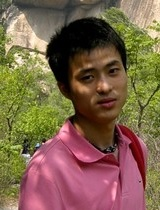
\includegraphics[width=1in,height=1.25in,clip,keepaspectratio]{figures/Peng_ForPaper.jpg}}]{Yi Peng}
is currently a Ph.D. student in Department of Computer Science and Technology at Tsinghua University.
He received his B.S. in school of software from the Tsinghua University, China, in 2010.
His research interests include scientific visualization, image processing, parallel computing and computer graphics.
\end{IEEEbiography}

\begin{IEEEbiography}[{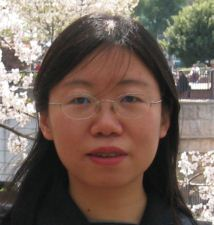
\includegraphics[width=1in,height=1.25in,clip,keepaspectratio]{figures/Chen_ForPaper.jpg}}]{Li Chen}
received the PhD degree in visualization from Zhejiang University in 1996.
Currently, she is an associate professor in the institute of CG \& CAD, School of Software, Tsinghua University.
Her research interests include data visualization, mesh generation and parallel algorithm.
\end{IEEEbiography}

\begin{IEEEbiography}[{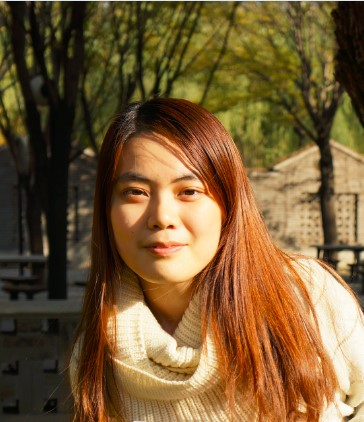
\includegraphics[width=1in,height=1.25in,clip,keepaspectratio]{figures/OuYang_ForPaper.jpg}}]{Fang-Xin Ou-Yang}
is currently a undergraduate student in School of Software, Tsinghua University.
Her research interests include visualization and computer graphics.
\end{IEEEbiography}

\begin{IEEEbiography}[{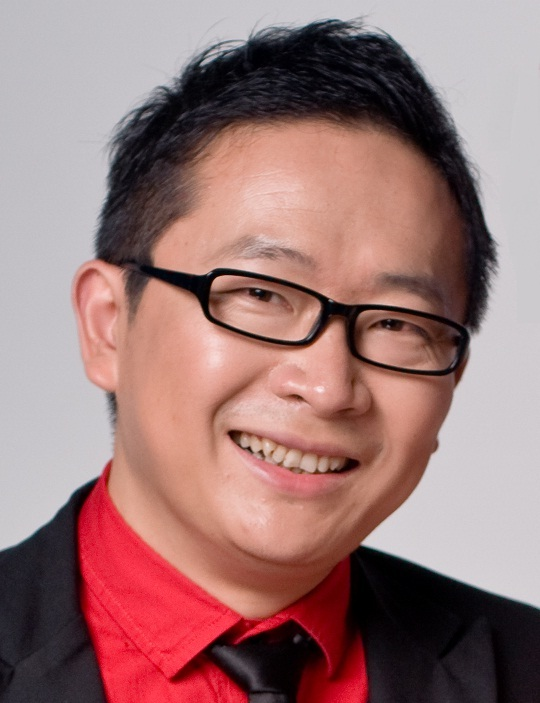
\includegraphics[width=1in,height=1.25in,clip,keepaspectratio]{figures/ChenWei_ForPaper.JPG}}]{Wei Chen}
Dr. Wei Chen is a professor in State Key Lab of CAD \& CG at Zhejiang University, P.R.China.
From June 2000 to June 2002, he was a joint Ph.D student in Fraunhofer Institute for Graphics, Darmstadt, Germany and received his Ph.D degree in July 2002.
His Ph.D advisors were Prof. Qunsheng Peng, and Prof. Georgios Sakas.
From July. 2006 to Sep. 2008, Dr. Wei Chen was a visiting scholar at Purdue University, working in PURPL with Prof.David S. Ebert.
In December 2009, Dr.Wei Chen was promoted as a full professor of Zhejiang University.
He has performed research in computer graphics and visualization and published more than 60 peer-reviewed journal and conference papers in the last five years.
His current research interests include visualization, visual analytics and bio-medical image computing.
\end{IEEEbiography}

\begin{IEEEbiography}[{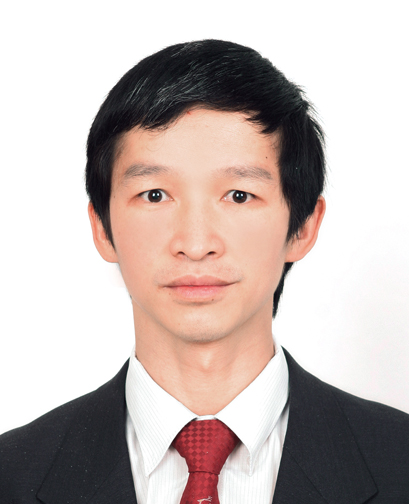
\includegraphics[width=1in,height=1.25in,clip,keepaspectratio]{figures/Yong_ForPaper.JPG}}]{Jun-Hai Yong}
is currently a professor in School of Software at Tsinghua University.
He received his B.S. and Ph.D. in computer science from the Tsinghua University, China, in 1996 and 2001, respectively.
He held a visiting researcher position in the Department of Computer Science at Hong Kong University of Science \& Technology in 2000.
He was a post doctoral fellow in the Department of Computer Science at the University of Kentucky from 2000 to 2002.
He obtained a lot of awards such as the National Excellent Doctoral Dissertation Award, the National Science Fund for Distinguished Young Scholars, the Best Paper Award of the ACM SIGGRAPH / Eurographics Symposium on Computer Animation, the Outstanding Service Award as Associate Editor of the Computers \& Graphics Journal by Elsevier, and several National Excellent Textbook Awards. His main research interests include computer-aided design and computer graphics.
\end{IEEEbiography}

% You can push biographies down or up by placing
% a \vfill before or after them. The appropriate
% use of \vfill depends on what kind of text is
% on the last page and whether or not the columns
% are being equalized.

%\vfill

% Can be used to pull up biographies so that the bottom of the last one
% is flush with the other column.
%\enlargethispage{-5in}



% that's all folks
\end{document}



